\section{Рабочий проект}
\subsection{Маршруты приложения}
В таблице \ref{routes:table} показаны маршруты приложения.

\begin{small}
\begin{xltabular}{\textwidth}{|X|c|c|}
	\caption{\label{routes:table}Маршруты приложения} \\ \hline
	\thead {URI} & \thead {HTTP-метод} & \thead {Метод контроллера} \\ \hline
	\endfirsthead
	\continuecaption{Продолжение таблицы \ref{routes:table}}
	\thead {URI} & \thead {HTTP-метод} & \thead {Метод контроллера} \\ \hline
	\finishhead
	/ & GET|HEAD & MainController@Index \\ \hline
	/admin/categories & GET|HEAD & Admin/CategoryController@index \\ \hline
	/admin/categories & POST & Admin/CategoryController@store \\ \hline
	/admin/categories/create  & GET|HEAD & Admin/CategoryController@create\\ \hline
	/admin/categories/ \{category\}  & GET|HEAD & Admin/CategoryController@show \\ \hline
	/admin/categories/ \{category\} & PUT|PATCH & Admin/CategoryController@update \\ \hline
	/admin/categories/ \{category\} & DELETE & Admin/CategoryController@destroy \\ \hline
	/admin/categories/ \{category\}/edit & GET|HEAD & Admin/CategoryController@edit \\ \hline
	/admin/orders  & GET|HEAD & Admin/OrderController@index \\ \hline
	/admin/orders/\{order\}  & GET|HEAD & Admin/OrderController@show \\ \hline
	/admin/ plants & GET|HEAD & Admin/PlantController@index \\ \hline
	/admin/ plants & POST & Admin/PlantController@store \\ \hline
	/admin/plants/create  & GET|HEAD & Admin/PlantController@create\\ \hline
	/admin/plants/\{plant\}  & GET|HEAD & Admin/PlantController@show  \\ \hline
	/admin/plants/\{plant\}  & PUT|PATCH & Admin/PlantController@update \\ \hline
	/admin/plants/\{plant\} & DELETE & Admin/PlantController@destroy \\ \hline
	/admin/plants/\{plant\}/edit & GET|HEAD & Admin/PlantController@edit   \\ \hline
	/basket & GET|HEAD & BasketController@basket \\ \hline
	/basket/add/\{id\}& POST & BasketController@basketAdd \\ \hline
	/basket/place & GET|HEAD & BasketController@basketPlace \\ \hline
	/basket/place & POST & BasketController@basketConfirm  \\ \hline
	/basket/remove/\{id\}& POST & BasketController@basketRemove \\ \hline
	/categories & GET|HEAD & MainController@categories  \\ \hline
	/categories/\{category\}& GET|HEAD & MainController@category \\ \hline
	/products/\{product\}& GET|HEAD & MainController@product \\ \hline
	/home & GET|HEAD & HomeController@index \\ \hline
	/home/\{order\} & GET|HEAD & HomeController@order \\ \hline
	/login & GET|HEAD & Auth/LoginController@showLoginForm  \\ \hline
	/login & POST & Auth/LoginController@login  \\ \hline
	/logout & POST & Auth/LoginController@logout  \\ \hline
	/logout & GET|HEAD & Auth/LoginController@logout  \\ \hline
	/password/confirm & GET|HEAD & Auth/ConfirmPasswordController@showConfirmForm  \\ \hline
	/password/confirm & POST & Auth/ConfirmPasswordController@confirm  \\ \hline
	/password/email & POST & Auth/ForgotPasswordController@sendResetLinkEmail \\ \hline
	/password/reset & GET|HEAD & Auth/ForgotPasswordController@showLinkRequestForm  \\ \hline
	/password/reset & POST & Auth/ResetPasswordController@reset  \\ \hline
	/password/reset/\{token\} & GET|HEAD & Auth/ResetPasswordController@showResetForm  \\ \hline
	/register & GET|HEAD & Auth/RegisterController@showRegistrationForm  \\ \hline
	/register & POST & Auth/RegisterController@register  \\ \hline
	/admin/categories & GET|HEAD & Admin/CategoryController@index 
\end{xltabular}
\end{small}


\subsection{Спецификация контроллеров приложения}

В таблице \ref{contr1:table} приведено описание методов класса <<MainController>>.

\begin{xltabular}{\textwidth}{|c|c|X|}
	\caption{\label{contr1:table}Спецификация методов класса <<MainController>>} \\ \hline
	\thead {Название} & \thead {Доступ} & \thead {Описание}\\ \hline
	\endfirsthead
	\continuecaption{Продолжение таблицы \ref{contr1:table}}
	\thead {Название} & \thead {Доступ} & \thead {Описание}\\ \hline
	\finishhead
	index & public & Выводит представление для главной страницы \\ \hline 
	categories & public & Выводит представление для категорий \\ \hline 
	category & public & Выводит представление для категории \\ \hline
	product & public & Выводит представление для товара
\end{xltabular}


В таблице \ref{contr2:table} приведено описание методов класса <<HomeController>>.

\begin{xltabular}{\textwidth}{|c|c|X|}
	\caption{\label{contr2:table}Спецификация методов класса <<HomeController>>} \\ \hline
	\thead {Название} & \thead {Доступ} & \thead {Описание}\\ \hline
	\endfirsthead
	\continuecaption{Продолжение таблицы \ref{contr2:table}}
	\thead {Название} & \thead {Доступ} & \thead {Описание}\\ \hline
	\finishhead
	\_\_construct & public & Устанавливает доступ только для зарегистрированных пользователей \\ \hline 
	index & public & Выводит представление для заказов пользователя\\ \hline 
	order & public & Выводит представление для заказа пользователя
\end{xltabular}


В таблице \ref{contr3:table} приведено описание методов класса <<BasketController>>.

\begin{xltabular}{\textwidth}{|c|c|X|}
	\caption{\label{contr3:table}Спецификация методов класса <<BasketController>>} \\ \hline
	\thead {Название} & \thead {Доступ} & \thead {Описание}\\ \hline
	\endfirsthead
	\continuecaption{Продолжение таблицы \ref{contr3:table}}
	\thead {Название} & \thead {Доступ} & \thead {Описание}\\ \hline
	\finishhead
	basket & public & Выводит представление для корзины \\ \hline 
	basketPlace & public & Выводит представление для оформления заказа \\ \hline
	basketConfirm & public & Сохраняет данные заказа и переносит пользователя на главную страницу после оформления заказа \\ \hline 
	basketAdd & public & Добавляет товар в корзину \\ \hline
	basketRemove & public & Удаляет товар из корзины
\end{xltabular}


Далее будет представлена спецификация контроллеров, находящихся в папке <<Admin>>.

В таблице \ref{contr4:table} приведено описание методов класса <<CategoryController>>.

\begin{xltabular}{\textwidth}{|c|c|X|}
	\caption{\label{contr4:table}Спецификация методов класса <<CategoryController>>} \\ \hline
	\thead {Название} & \thead {Доступ} & \thead {Описание}\\ \hline
	\endfirsthead
	\continuecaption{Продолжение таблицы \ref{contr4:table}}
	\thead {Название} & \thead {Доступ} & \thead {Описание}\\ \hline
	\finishhead
	index & public & Выводит представление для категорий в панели администратора \\ \hline 
	create & public & Выводит представление для создания категории \\ \hline 
	store & public & Сохраняет категорию в базу данных \\ \hline
	show & public & Выводит представление для категории в панели администратора \\ \hline
	edit & public & Выводит представление для редактирования категории \\ \hline
	update & public & Обновляет информацию о категории в базе данных \\ \hline
	destroy & public & Удаляет категорию из базы данных
\end{xltabular}


В таблице \ref{contr5:table} приведено описание методов класса <<OrderController>>.

\begin{xltabular}{\textwidth}{|c|c|X|}
	\caption{\label{contr5:table}Спецификация методов класса <<OrderController>>} \\ \hline
	\thead {Название} & \thead {Доступ} & \thead {Описание}\\ \hline
	\endfirsthead
	\continuecaption{Продолжение таблицы \ref{contr5:table}}
	\thead {Название} & \thead {Доступ} & \thead {Описание}\\ \hline
	\finishhead
	index & public & Выводит представление для заказов в панели администратора \\ \hline 
	show & public & Выводит представление для заказа в панели администратора 
\end{xltabular}


В таблице \ref{contr6:table} приведено описание методов класса <<PlantController>>.

\begin{xltabular}{\textwidth}{|c|c|X|}
	\caption{\label{contr6:table}Спецификация методов класса <<PlantController>>} \\ \hline
	\thead {Название} & \thead {Доступ} & \thead {Описание}\\ \hline
	\endfirsthead
	\continuecaption{Продолжение таблицы \ref{contr6:table}}
	\thead {Название} & \thead {Доступ} & \thead {Описание}\\ \hline
	\finishhead
	index & public & Выводит представление для товаров в панели администратора \\ \hline 
	create & public & Выводит представление для создания товара \\ \hline 
	store & public & Сохраняет товар в базу данных \\ \hline
	show & public & Выводит представление для товара в панели администратора \\ \hline
	edit & public & Выводит представление для редактирования товара \\ \hline
	update & public & Обновляет информацию о товаре в базе данных \\ \hline
	destroy & public & Удаляет товар из базы данных
\end{xltabular}



Далее будет представлена спецификация контроллеров, находящихся в папке <<Auth>>.

В таблице \ref{contr7:table} приведено описание методов класса <<ConfirmPasswordController>>.

\begin{xltabular}{\textwidth}{|c|c|X|}
	\caption{\label{contr7:table}Спецификация методов класса <<ConfirmPasswordController>>} \\ \hline
	\thead {Название} & \thead {Доступ} & \thead {Описание}\\ \hline
	\endfirsthead
	\continuecaption{Продолжение таблицы \ref{contr7:table}}
	\thead {Название} & \thead {Доступ} & \thead {Описание}\\ \hline
	\finishhead
	\_\_construct & public & Разрешает доступ только авторизованным пользователям
\end{xltabular}


В таблице \ref{contr8:table} приведено описание методов класса <<LoginController>>.

\begin{xltabular}{\textwidth}{|c|c|X|}
	\caption{\label{contr8:table}Спецификация методов класса <<LoginController>>} \\ \hline
	\thead {Название} & \thead {Доступ} & \thead {Описание}\\ \hline
	\endfirsthead
	\continuecaption{Продолжение таблицы \ref{contr8:table}}
	\thead {Название} & \thead {Доступ} & \thead {Описание}\\ \hline
	\finishhead
	redirectTo & protected & Переносит пользователя на другую страницу после входа \\ \hline 
	\_\_construct & public & Разрешает доступ только неавторизованным пользователям 
\end{xltabular}


В таблице \ref{contr9:table} приведено описание методов класса <<RegisterController>>.

\begin{xltabular}{\textwidth}{|c|c|X|}
	\caption{\label{contr9:table}Спецификация методов класса <<RegisterController>>} \\ \hline
	\thead {Название} & \thead {Доступ} & \thead {Описание}\\ \hline
	\endfirsthead
	\continuecaption{Продолжение таблицы \ref{contr9:table}}
	\thead {Название} & \thead {Доступ} & \thead {Описание}\\ \hline
	\finishhead
	redirectTo & protected & Переносит пользователя на другую страницу после регистрации \\ \hline 
	\_\_construct & public & Разрешает доступ только неавторизованным пользователям \\ \hline 
	validator & protected & Валидирует данные для регистрации пользователя \\ \hline
	create & protected & Сохраняет нового пользователя в базе данных
\end{xltabular}


В таблице \ref{contr10:table} приведено описание методов класса <<ResetPasswordController>>.

\begin{xltabular}{\textwidth}{|c|c|X|}
	\caption{\label{contr10:table}Спецификация методов класса <<ResetPasswordController>>} \\ \hline
	\thead {Название} & \thead {Доступ} & \thead {Описание}\\ \hline
	\endfirsthead
	\continuecaption{Продолжение таблицы \ref{contr10:table}}
	\thead {Название} & \thead {Доступ} & \thead {Описание}\\ \hline
	\finishhead
	redirectTo & protected & Переносит пользователя на другую страницу после сброса пароля \\ \hline
\end{xltabular}


В таблице \ref{contr11:table} приведено описание методов класса <<VerificationController>>.

\begin{xltabular}{\textwidth}{|c|c|X|}
	\caption{\label{contr11:table}Спецификация методов класса <<VerificationController>>} \\ \hline
	\thead {Название} & \thead {Доступ} & \thead {Описание}\\ \hline
	\endfirsthead
	\continuecaption{Продолжение таблицы \ref{contr11:table}}
	\thead {Название} & \thead {Доступ} & \thead {Описание}\\ \hline
	\finishhead
	redirectTo & protected & Переносит пользователя на другую страницу после верификации \\ \hline 
	\_\_construct & public & Разрешает доступ только авторизованным пользователям \\ \hline 
\end{xltabular}


\subsection{Системное тестирование разработанного web-сайта}

На рисунке \ref{index:image} показана главная страница сайта.

\begin{figure}[H]
	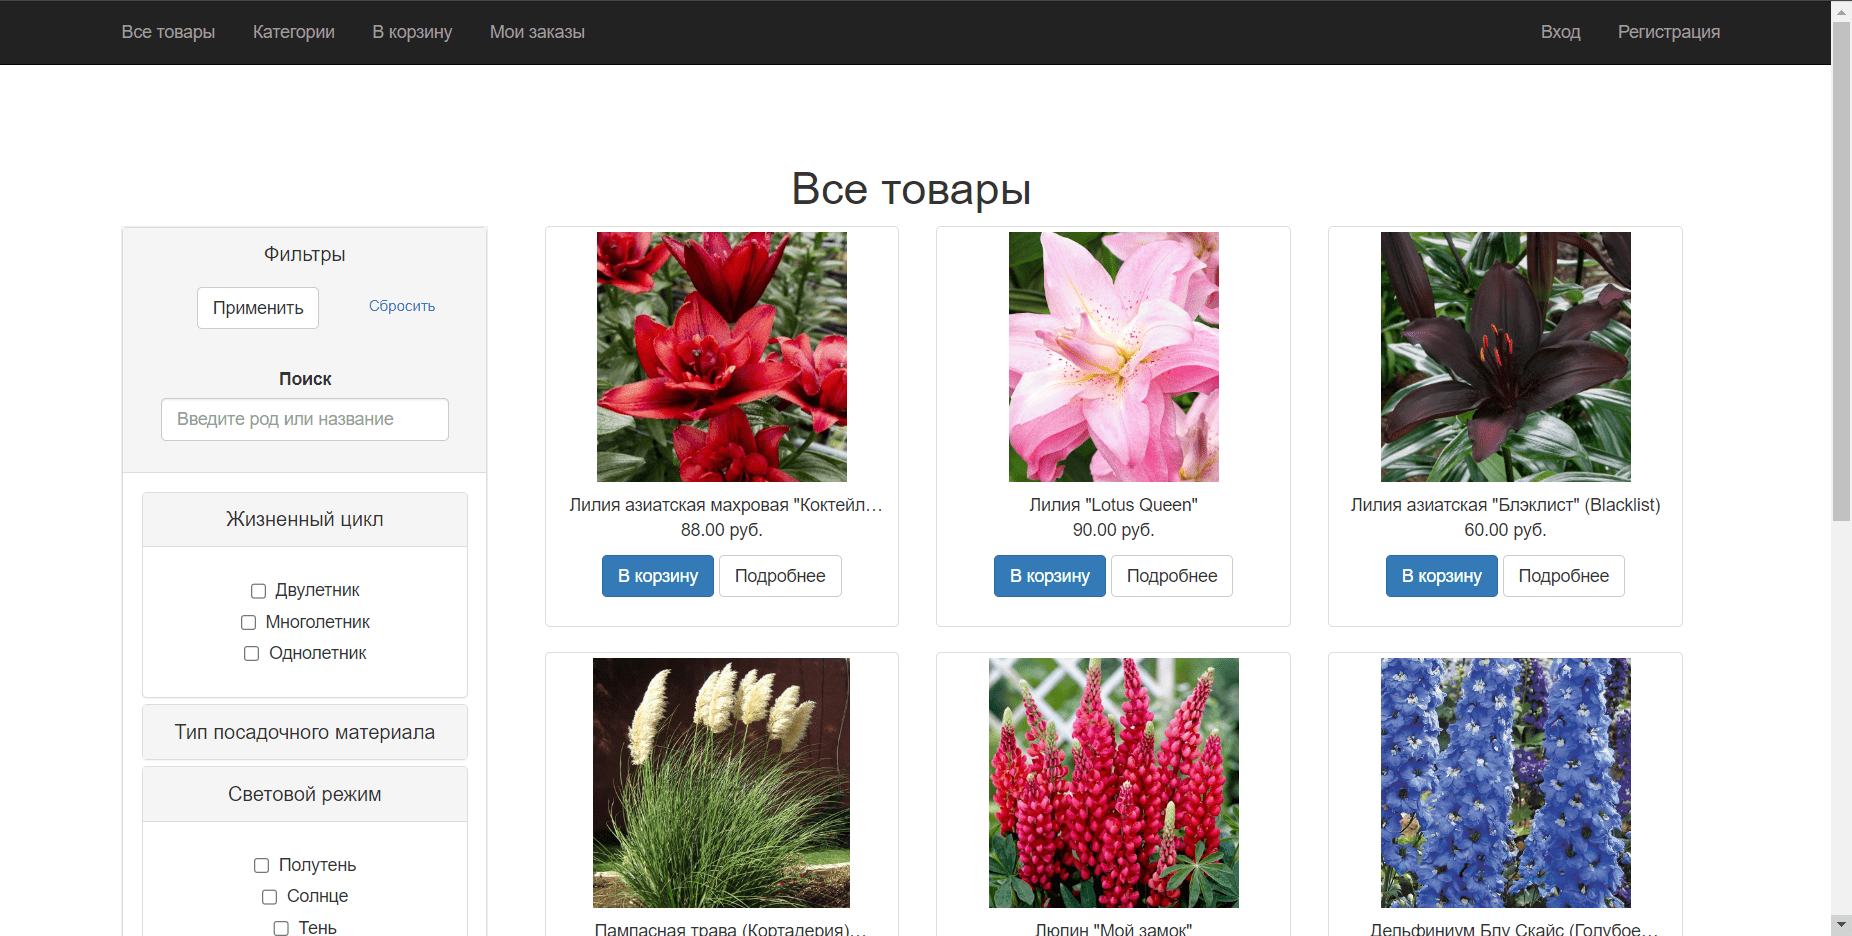
\includegraphics[width=1\linewidth]{index}
	\caption{Главная страница}
	\label{index:image}
\end{figure}
%\vspace{-\figureaboveskip} % двойной отступ не нужен (можно использовать, если раздел заканчивается картинкой)

На рисунке \ref{1filter:image} показан результат фильтрации товаров на главной странице по одному параметру.

\begin{figure}[H]
	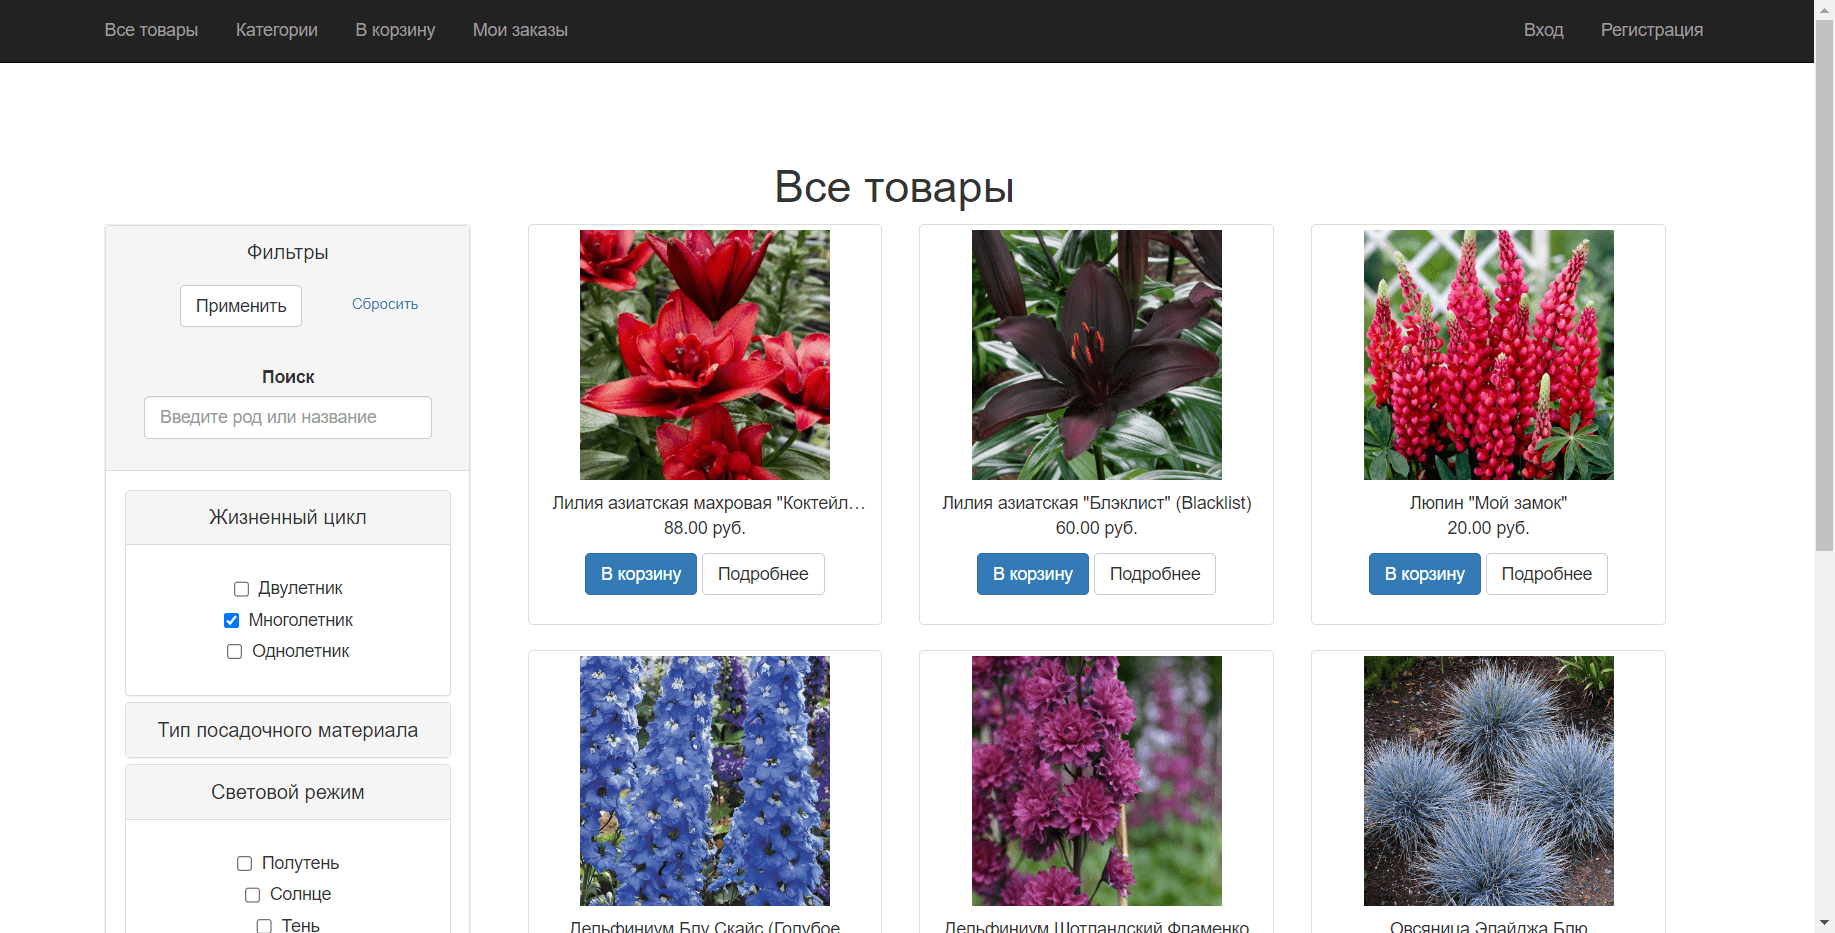
\includegraphics[width=1\linewidth]{1filter}
	\caption{Фильтрация по одному параметру}
	\label{1filter:image}
\end{figure}
%\vspace{-\figureaboveskip} % двойной отступ не нужен (можно использовать, если раздел заканчивается картинкой)

На рисунке \ref{2filter:image} показан результат фильтрации товаров на главной странице по нескольким параметрам.

\begin{figure}[H]
	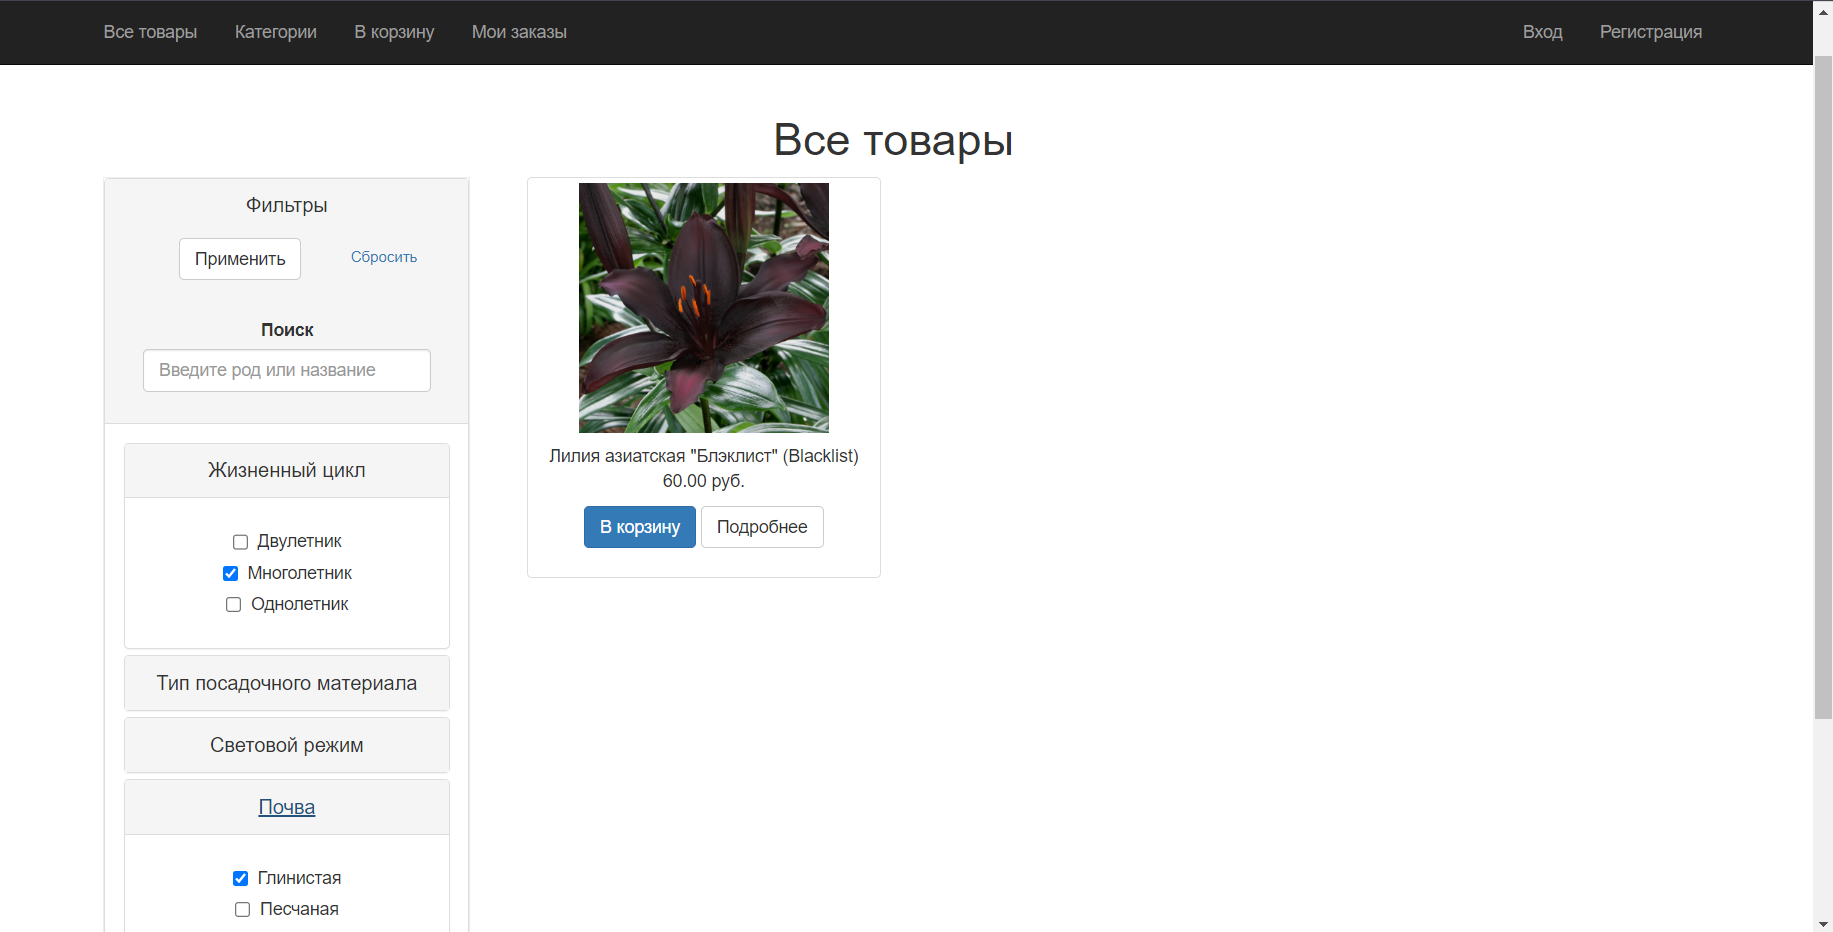
\includegraphics[width=1\linewidth]{2filter}
	\caption{Фильтрация по нескольким параметрам}
	\label{2filter:image}
\end{figure}
%\vspace{-\figureaboveskip} % двойной отступ не нужен (можно использовать, если раздел заканчивается картинкой)

На рисунке \ref{search:image} показан результат поиска товаров по названию.

\begin{figure}[H]
	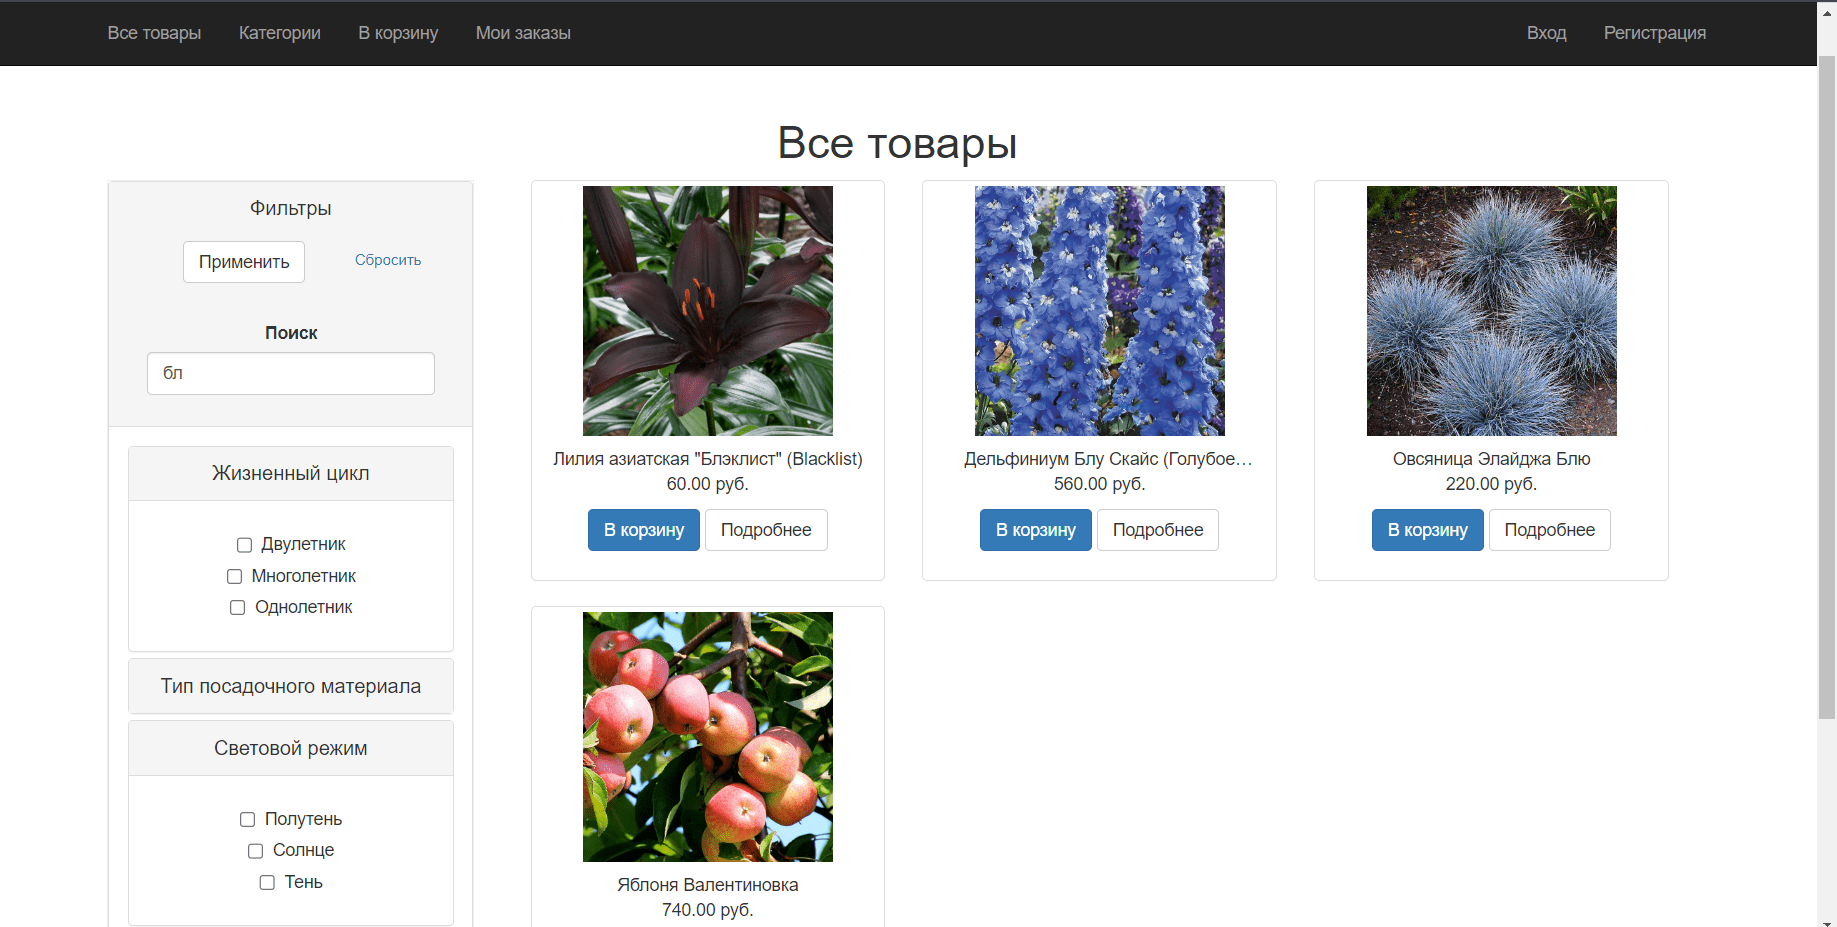
\includegraphics[width=1\linewidth]{search}
	\caption{Поиск по названию}
	\label{search:image}
\end{figure}
%\vspace{-\figureaboveskip} % двойной отступ не нужен (можно использовать, если раздел заканчивается картинкой)

На рисунке \ref{product:image} показана страница одного из товаров.

\begin{figure}[H]
	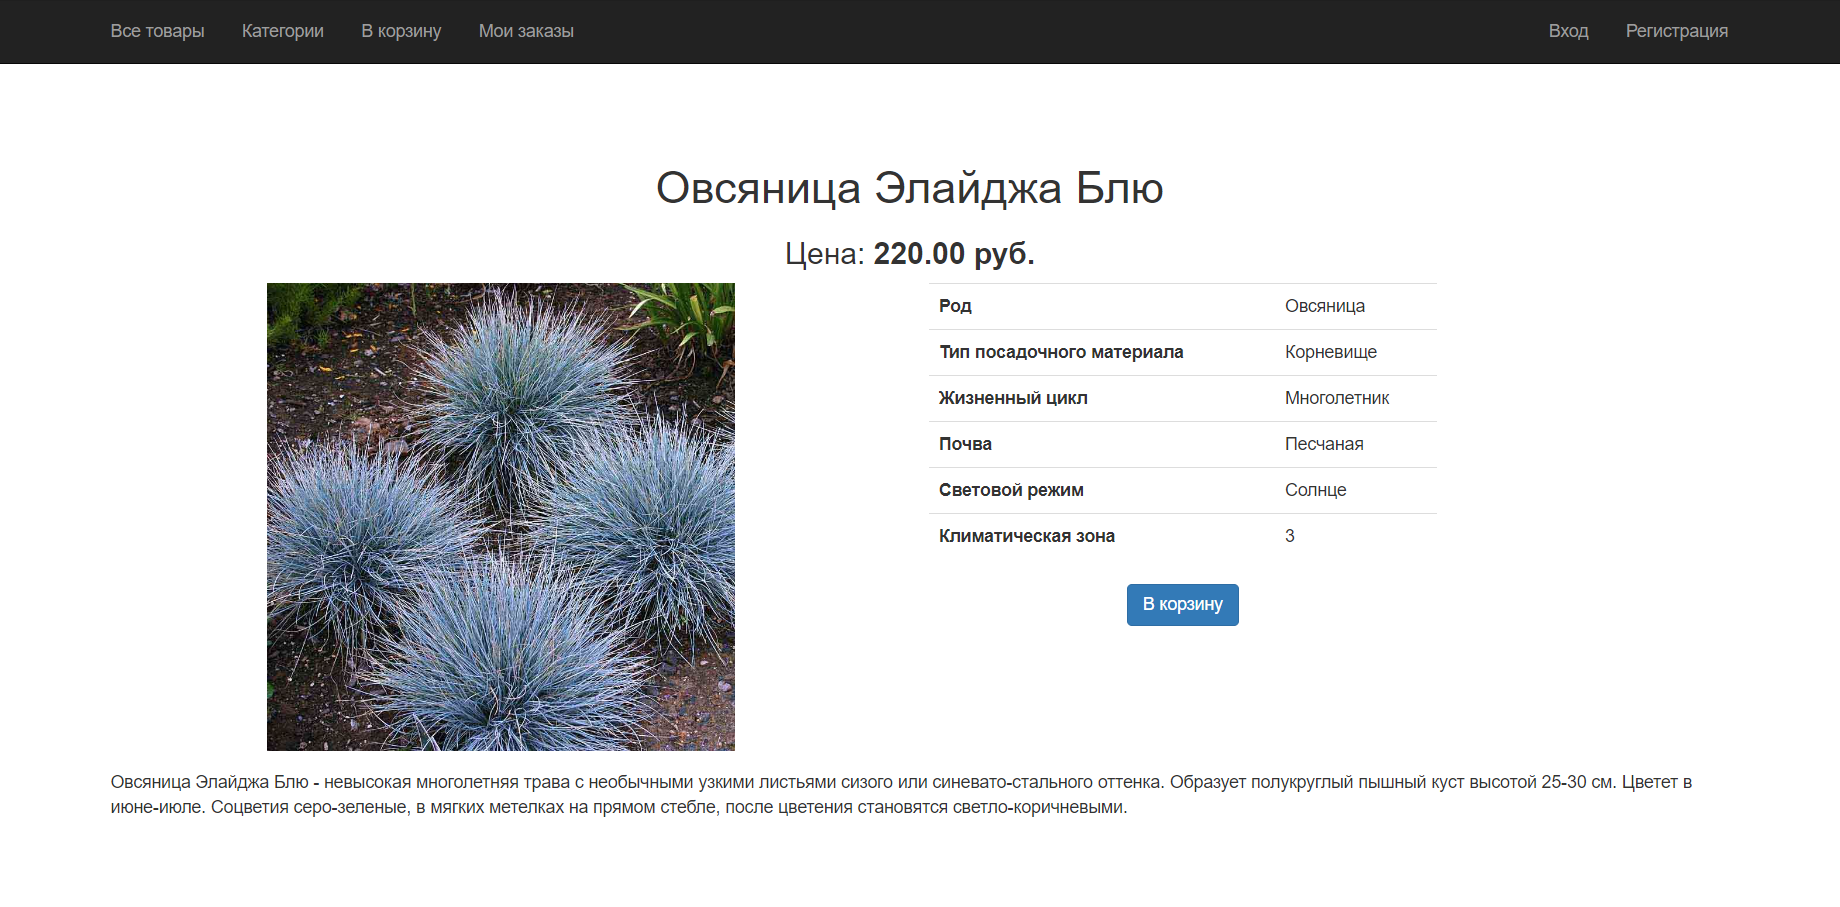
\includegraphics[width=1\linewidth]{product}
	\caption{Страница товара}
	\label{product:image}
\end{figure}
%\vspace{-\figureaboveskip} % двойной отступ не нужен (можно использовать, если раздел заканчивается картинкой)


На рисунке \ref{categories:image} показана страница категорий.

\begin{figure}[H]
	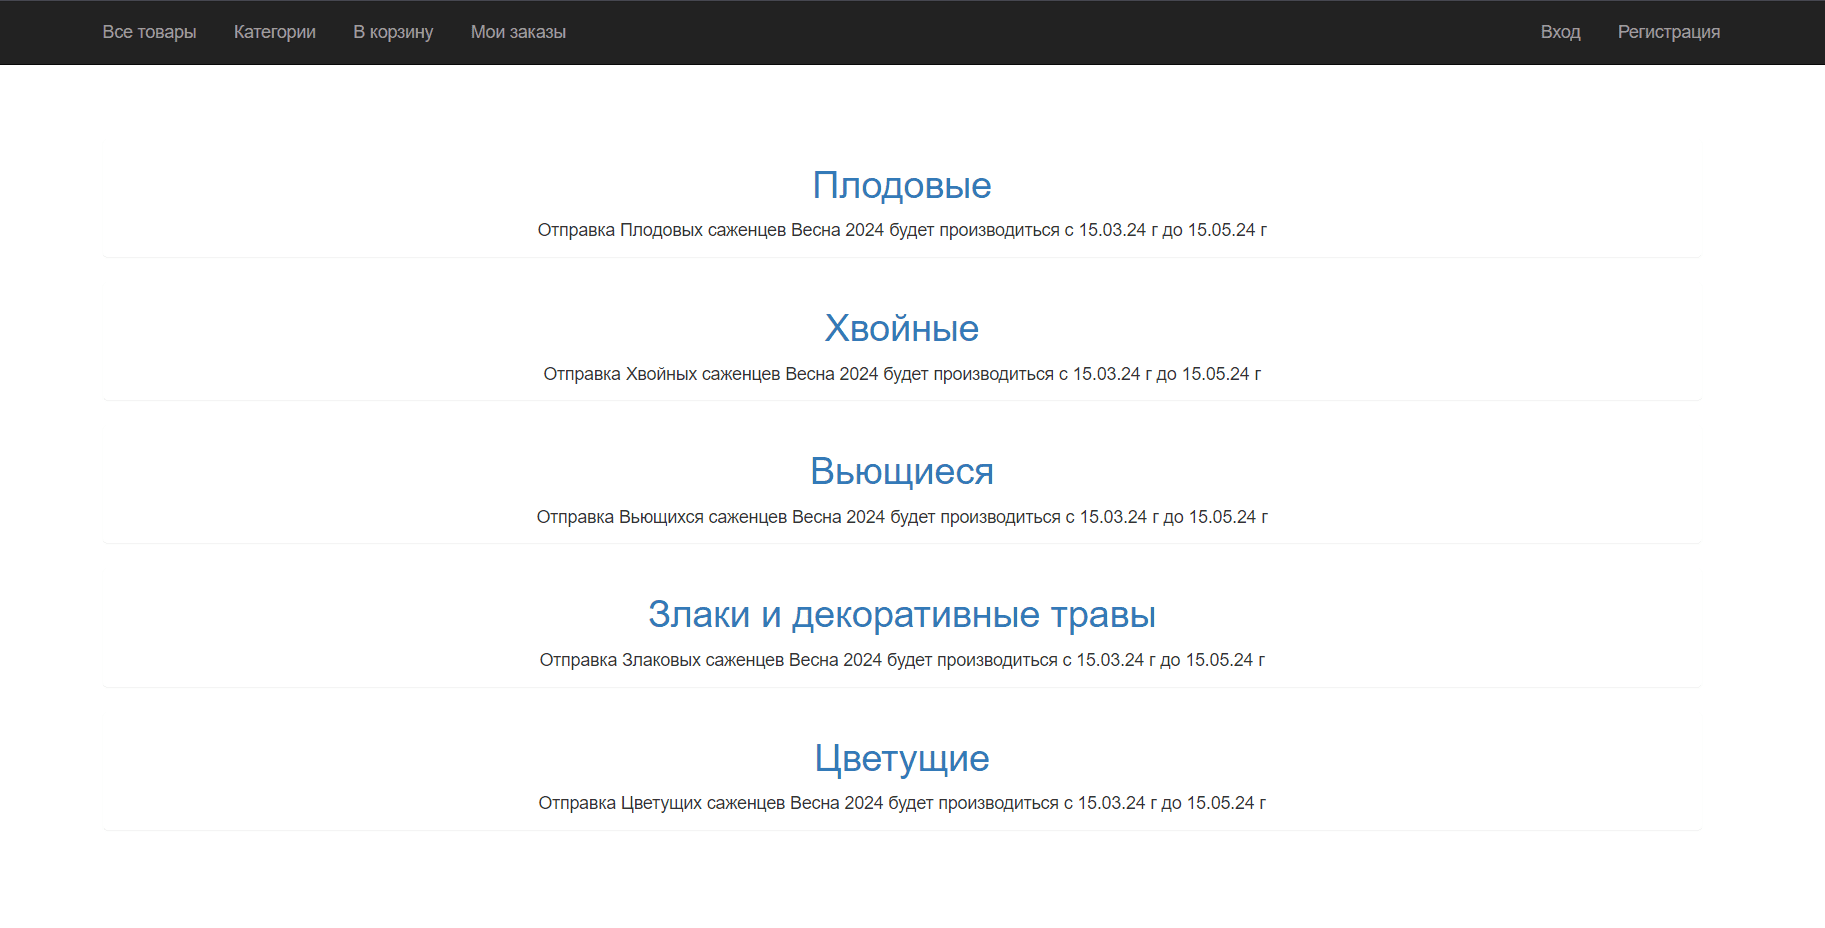
\includegraphics[width=1\linewidth]{categories}
	\caption{Страница категорий}
	\label{categories:image}
\end{figure}
%\vspace{-\figureaboveskip} % двойной отступ не нужен (можно использовать, если раздел заканчивается картинкой)


На рисунке \ref{category:image} показана страница категории <<Злаки и декоративные травы>>.

\begin{figure}[H]
	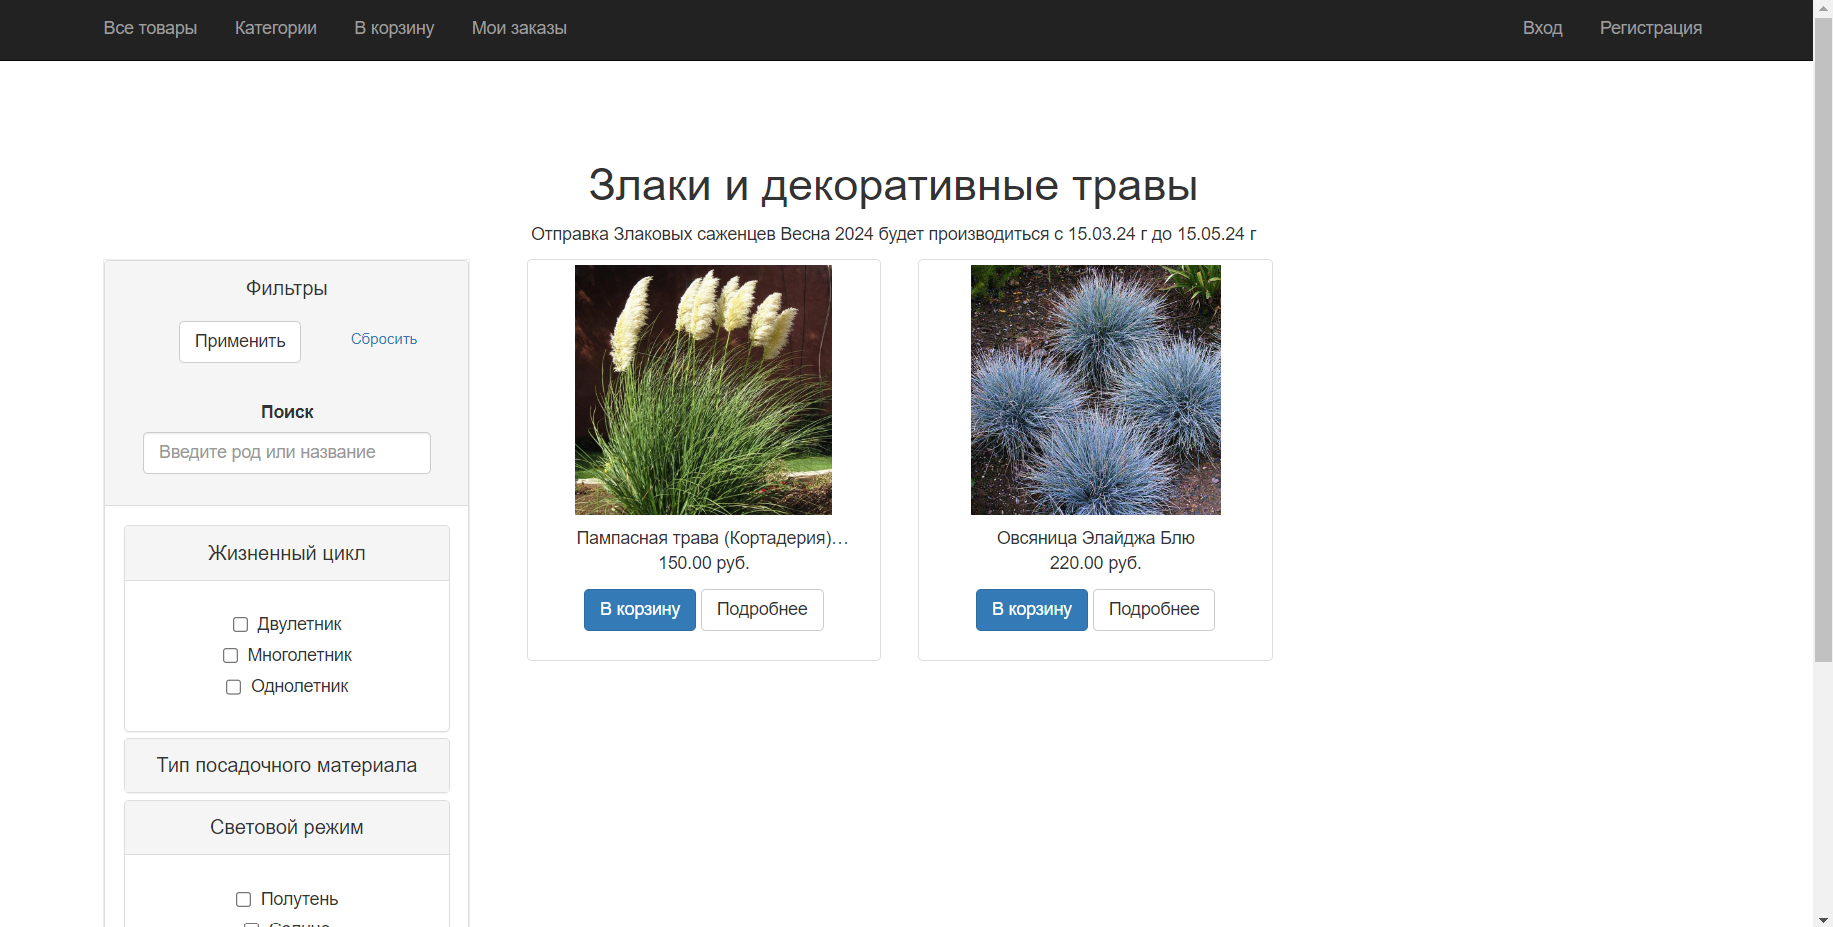
\includegraphics[width=1\linewidth]{category}
	\caption{Страница категории}
	\label{category:image}
\end{figure}
%\vspace{-\figureaboveskip} % двойной отступ не нужен (можно использовать, если раздел заканчивается картинкой)

После применения фильтрации на странице категории выведутся товары, принадлежащие этой категории и соответствующие выбранным значениям характеристик. Это показано на рисунке \ref{categoryFilter:image}.

\begin{figure}[H]
	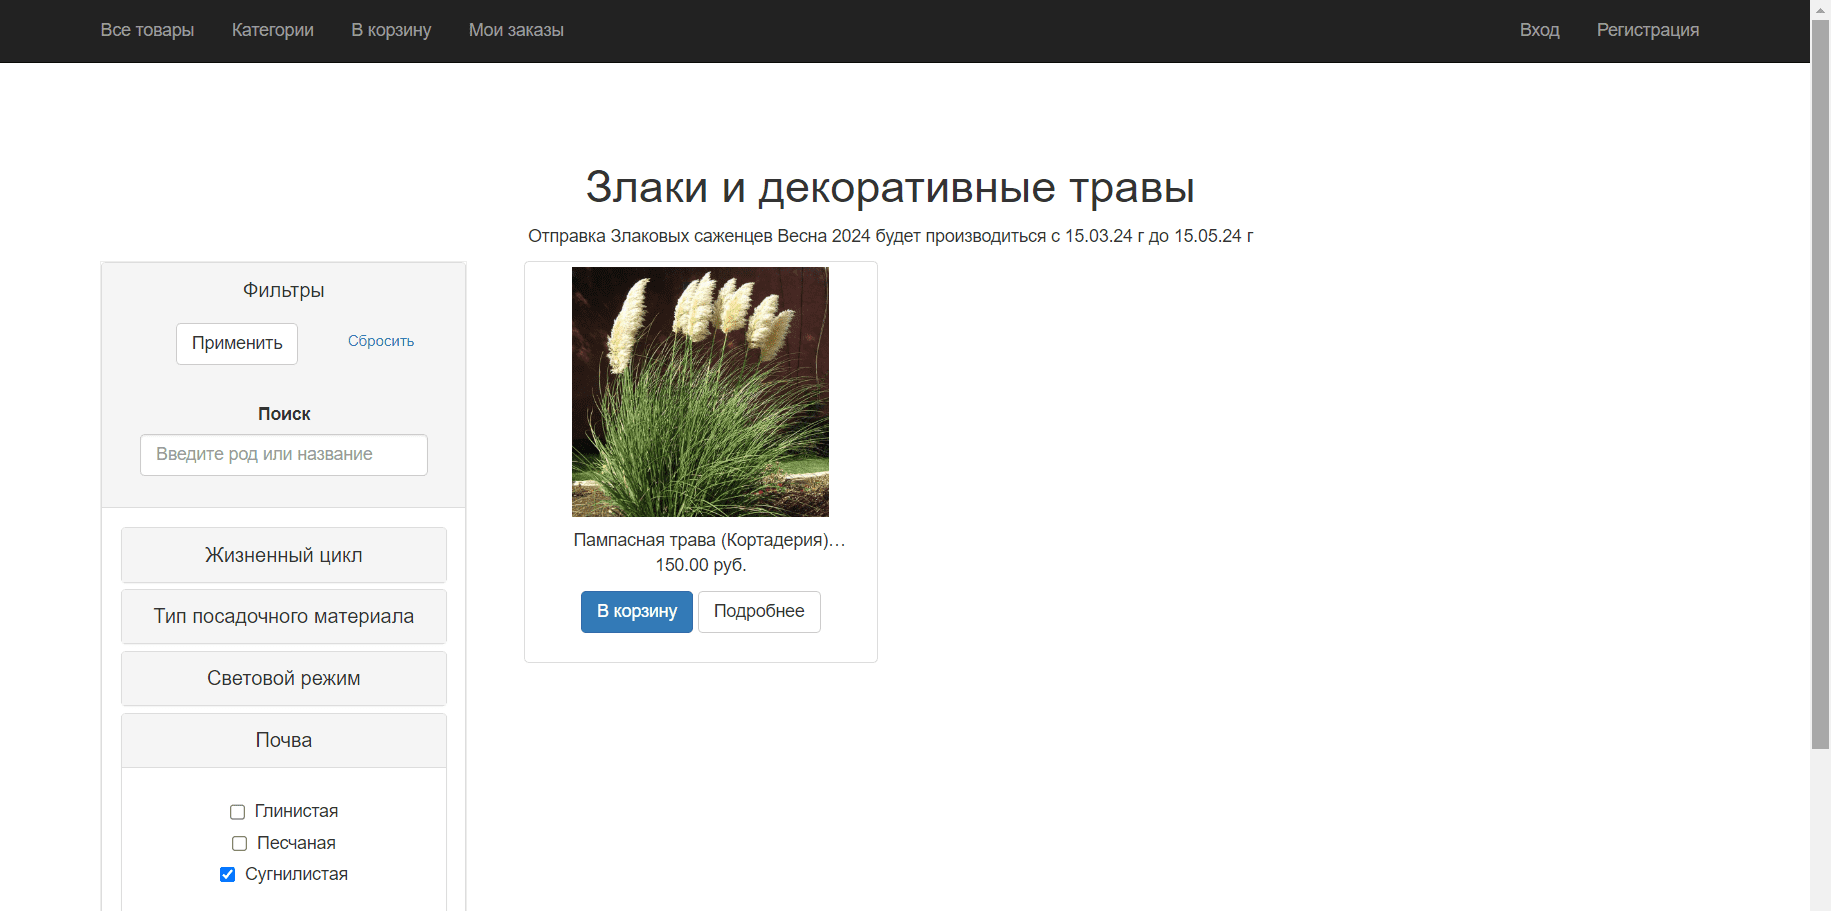
\includegraphics[width=1\linewidth]{categoryFilter}
	\caption{Фильтрация на странице категории}
	\label{categoryFilter:image}
\end{figure}
%\vspace{-\figureaboveskip} % двойной отступ не нужен (можно использовать, если раздел заканчивается картинкой)


На рисунке \ref{basketNull:image} показана корзина до добавления в неё товаров.

\begin{figure}[H]
	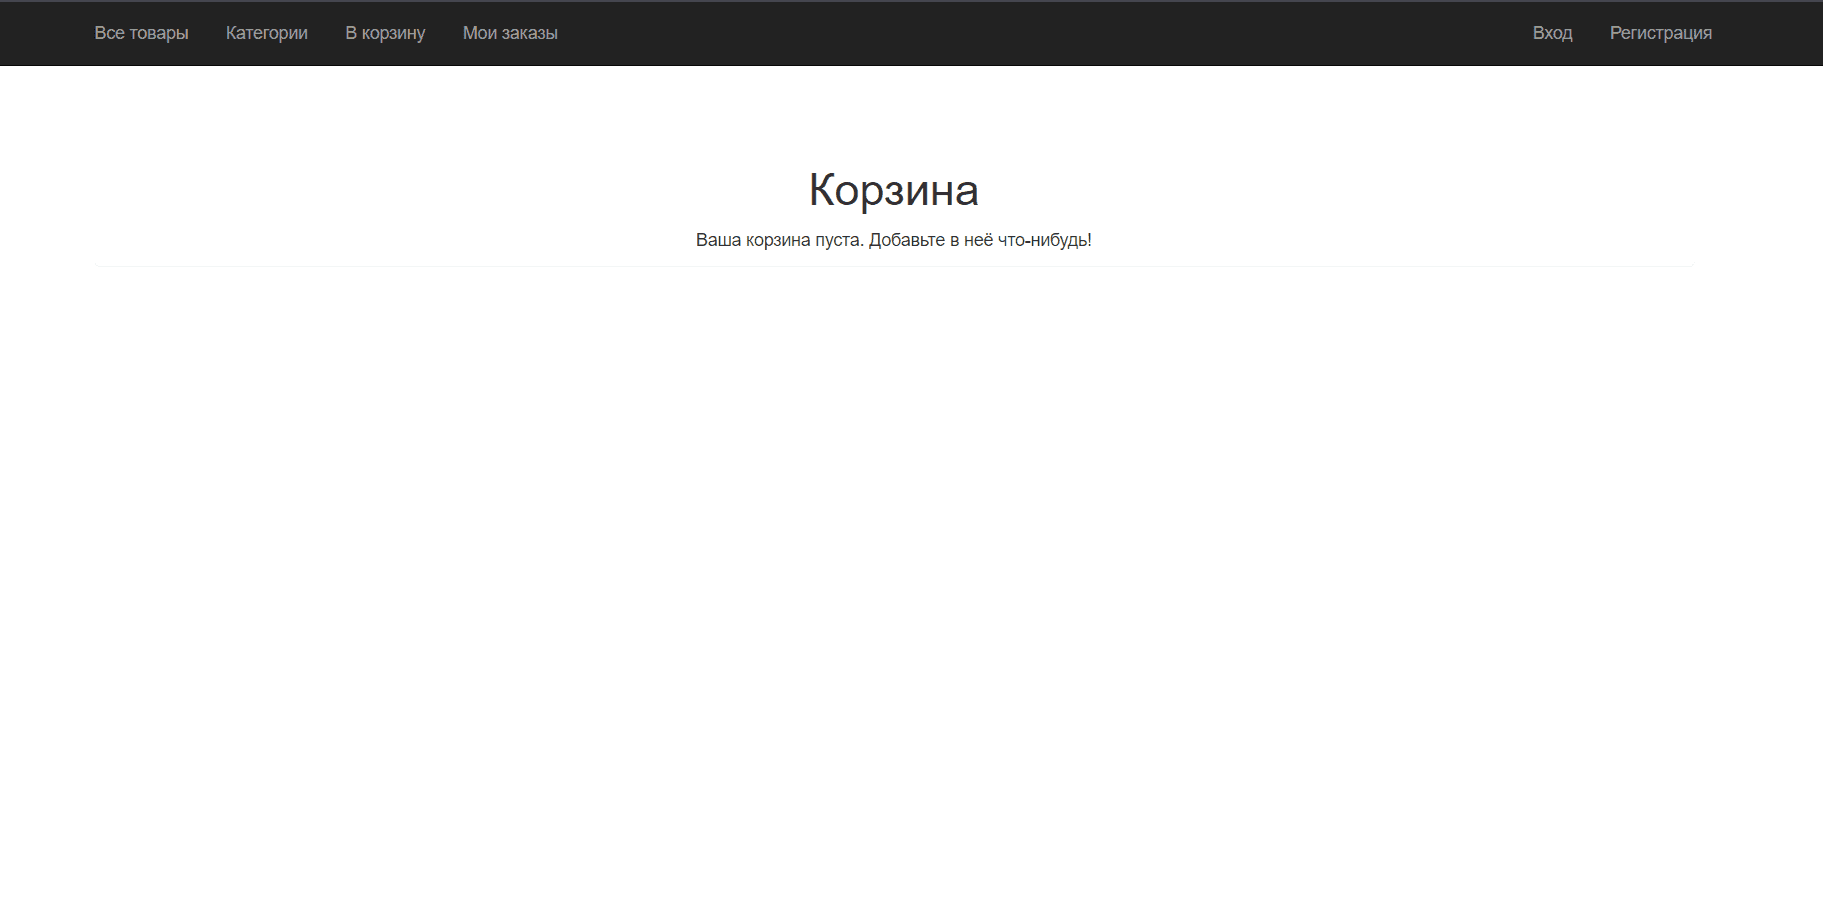
\includegraphics[width=1\linewidth]{basketNull}
	\caption{Пустая корзина}
	\label{basketNull:image}
\end{figure}
%\vspace{-\figureaboveskip} % двойной отступ не нужен (можно использовать, если раздел заканчивается картинкой)

На рисунке \ref{basketAdd:image} показано добавление товара в корзину.

\begin{figure}[H]
	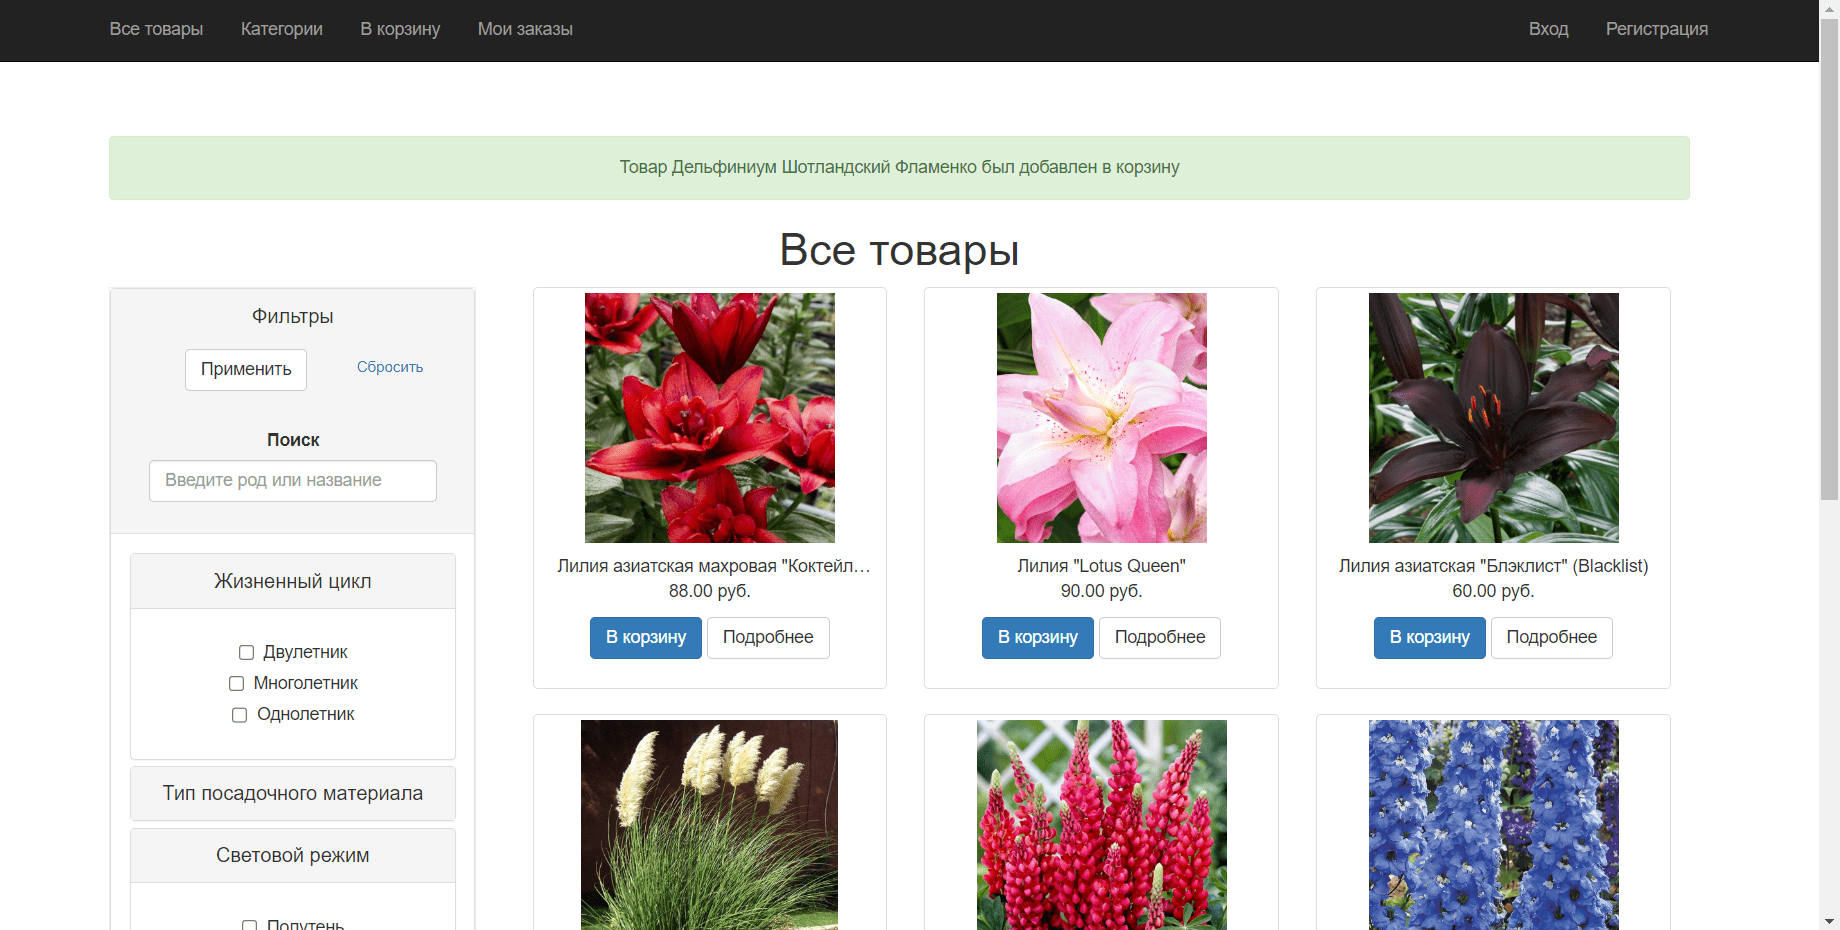
\includegraphics[width=1\linewidth]{basketAdd}
	\caption{Добавление товара в корзину}
	\label{basketAdd:image}
\end{figure}
%\vspace{-\figureaboveskip} % двойной отступ не нужен (можно использовать, если раздел заканчивается картинкой)

На рисунке \ref{basket:image} показана корзина с товарами.

\begin{figure}[H]
	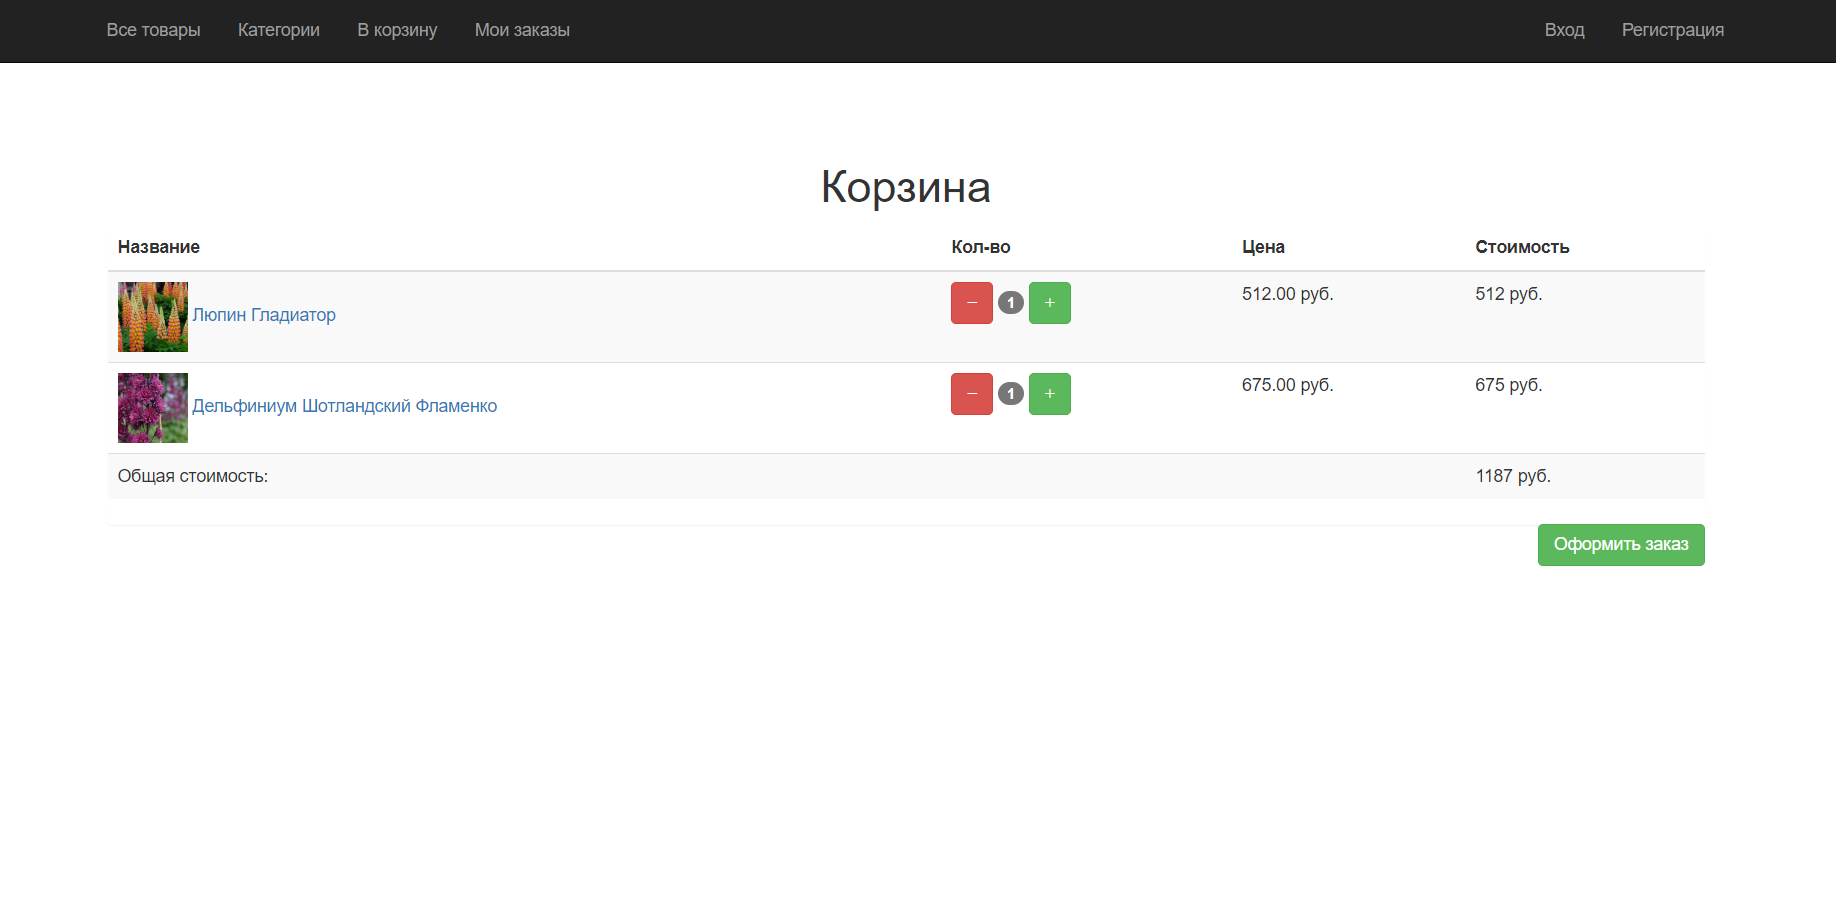
\includegraphics[width=1\linewidth]{basket}
	\caption{Корзина с товарами}
	\label{basket:image}
\end{figure}
%\vspace{-\figureaboveskip} % двойной отступ не нужен (можно использовать, если раздел заканчивается картинкой)

На рисунке \ref{basketRemove:image} показано удаление товара из корзины.

\begin{figure}[H]
	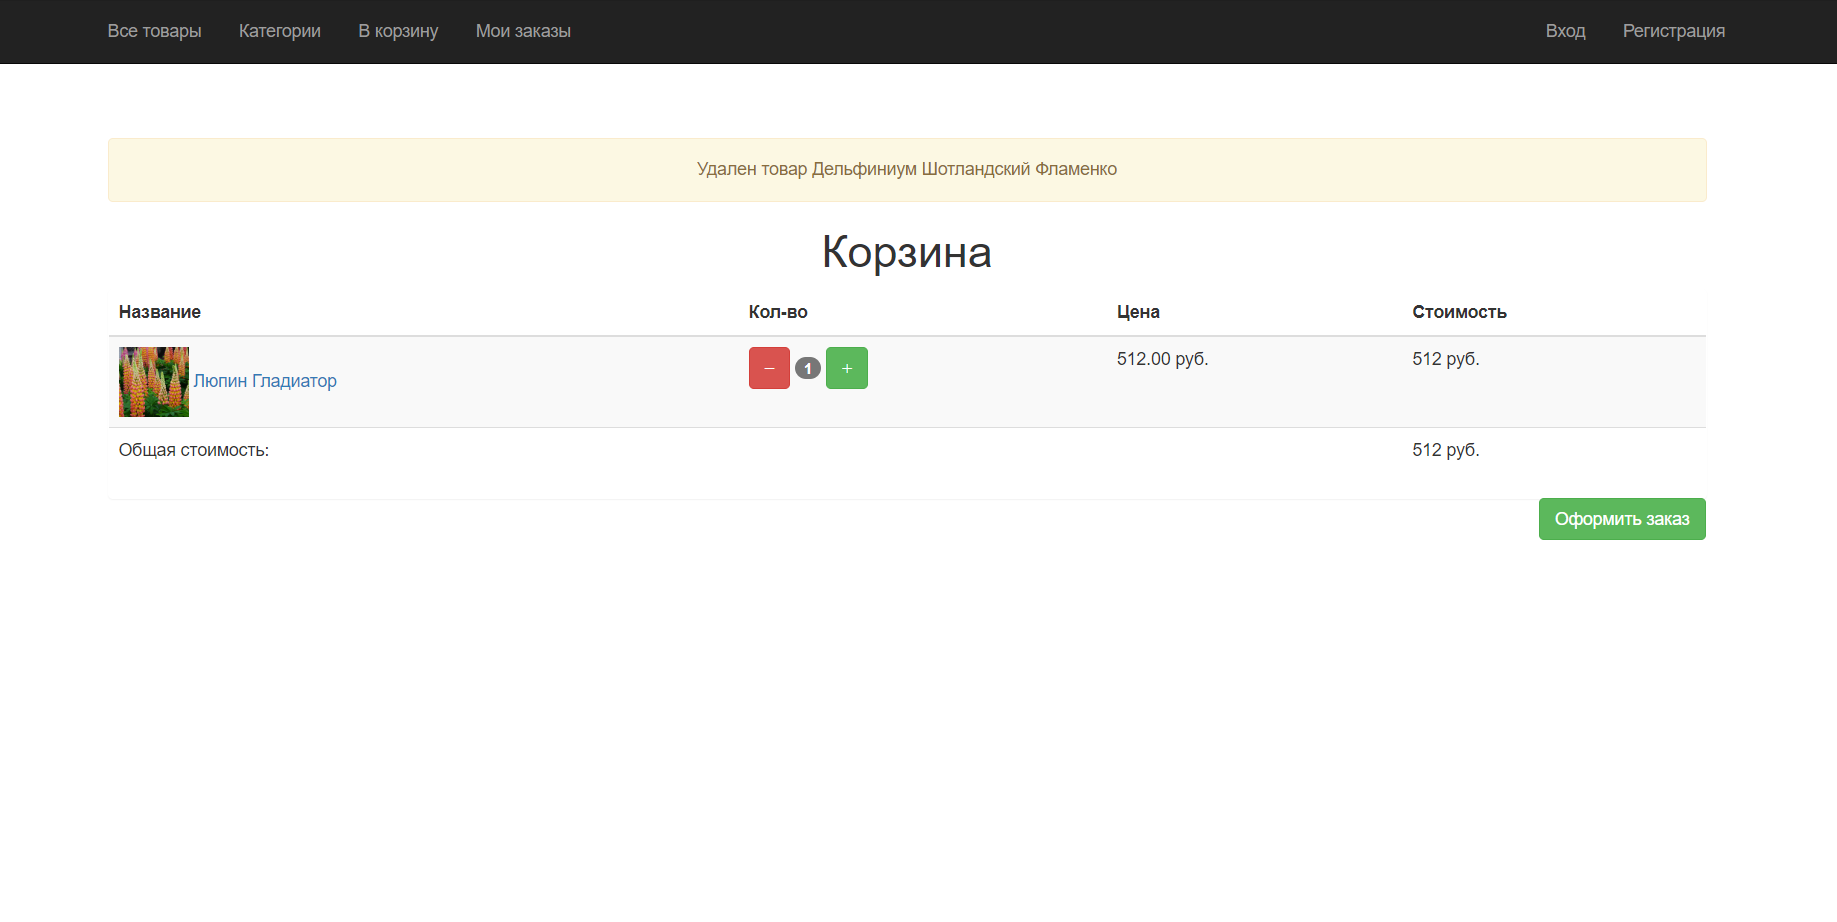
\includegraphics[width=1\linewidth]{basketRemove}
	\caption{Удаление товара из корзины}
	\label{basketRemove:image}
\end{figure}
%\vspace{-\figureaboveskip} % двойной отступ не нужен (можно использовать, если раздел заканчивается картинкой)

На рисунке \ref{confirm:image} показана страница оформления заказа.

\begin{figure}[H]
	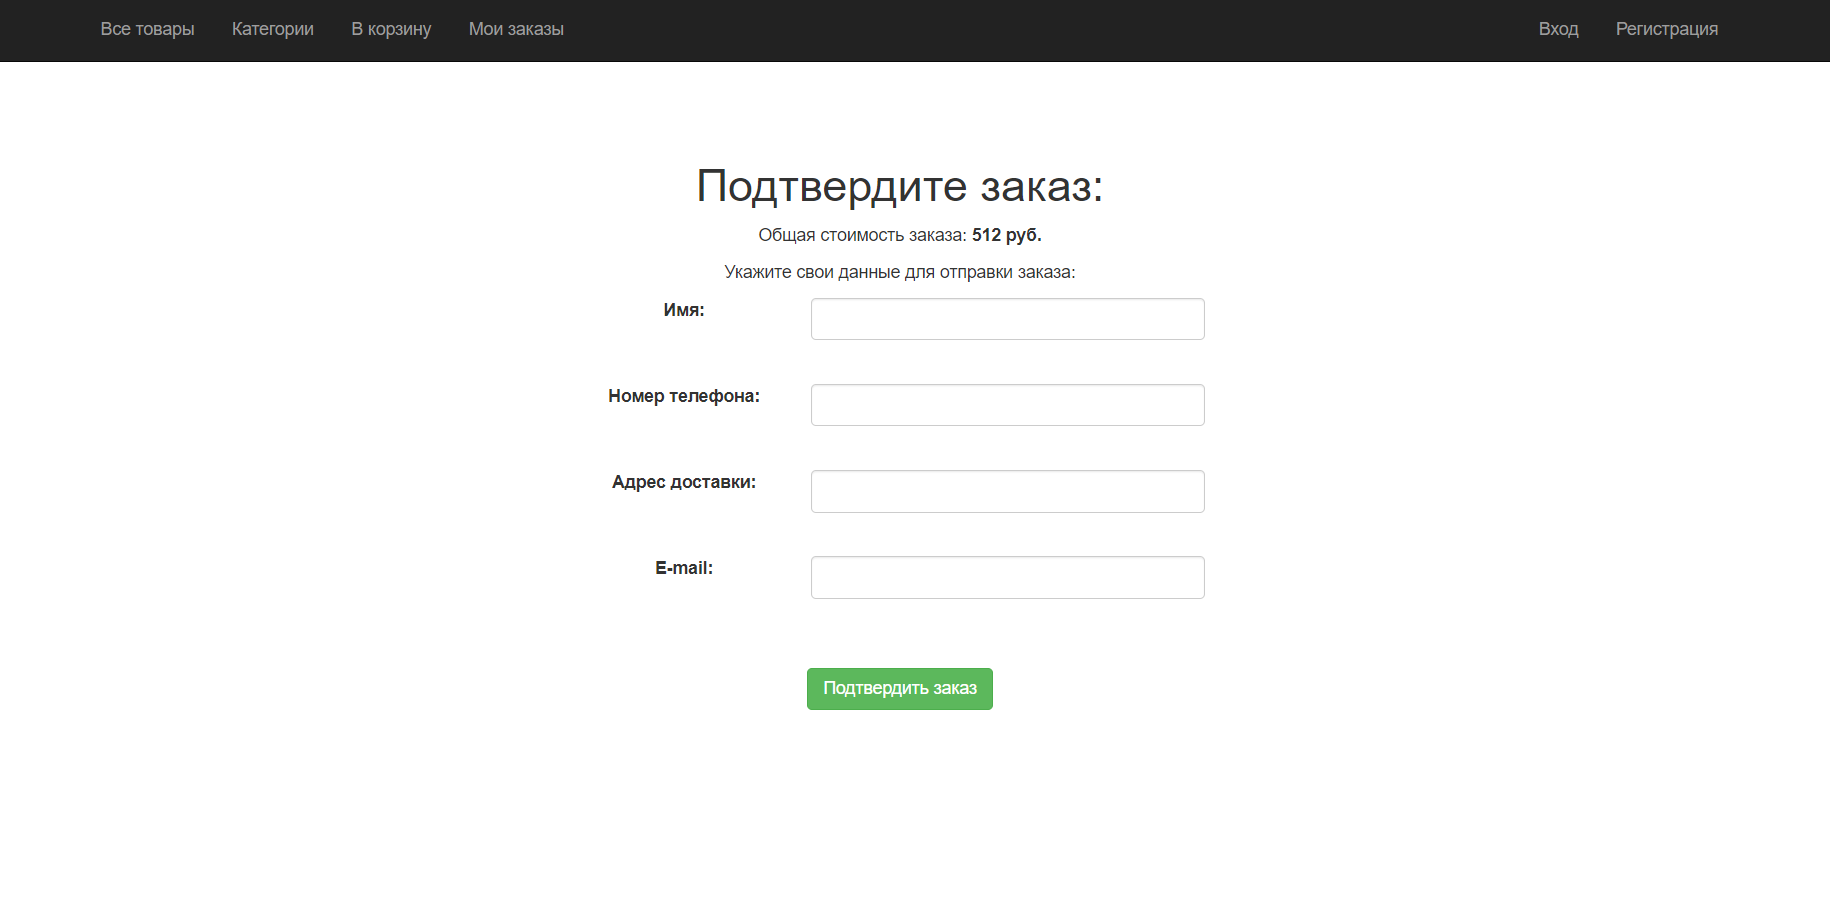
\includegraphics[width=1\linewidth]{confirm}
	\caption{Страница оформления заказа}
	\label{confirm:image}
\end{figure}
%\vspace{-\figureaboveskip} % двойной отступ не нужен (можно использовать, если раздел заканчивается картинкой)

На рисунке \ref{login:image} показана страница входа.

\begin{figure}[H]
	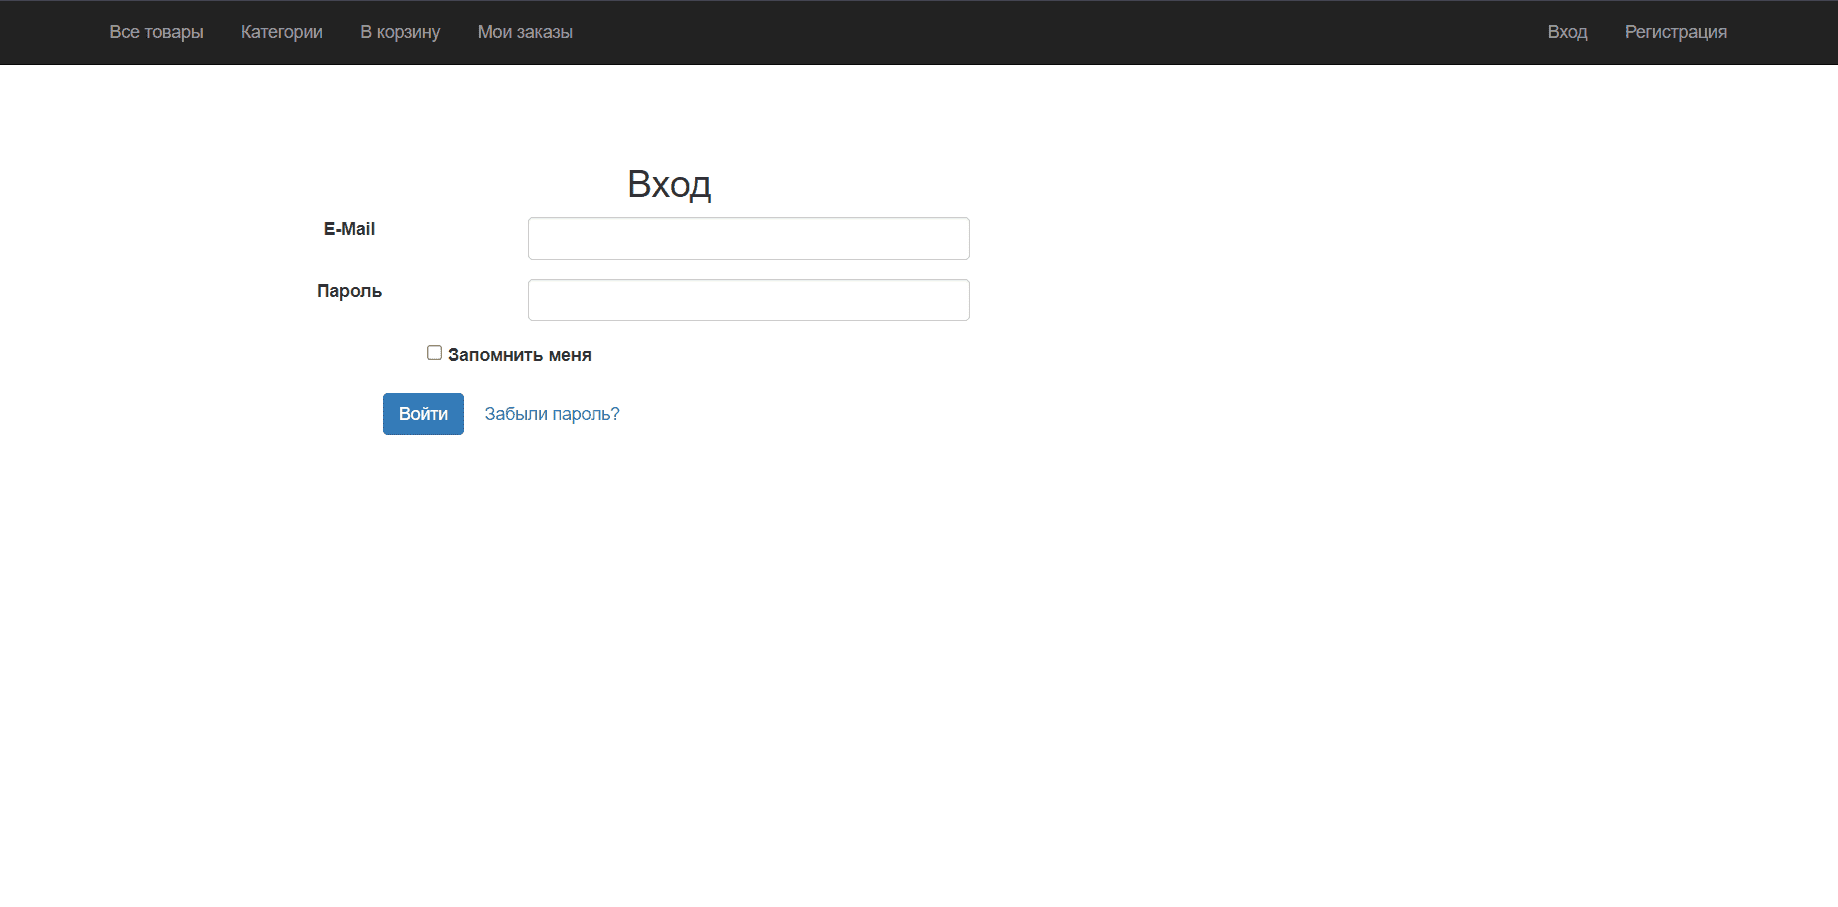
\includegraphics[width=1\linewidth]{login}
	\caption{Страница входа}
	\label{login:image}
\end{figure}
%\vspace{-\figureaboveskip} % двойной отступ не нужен (можно использовать, если раздел заканчивается картинкой)

На рисунке \ref{register:image} показана страница регистрации.

\begin{figure}[H]
	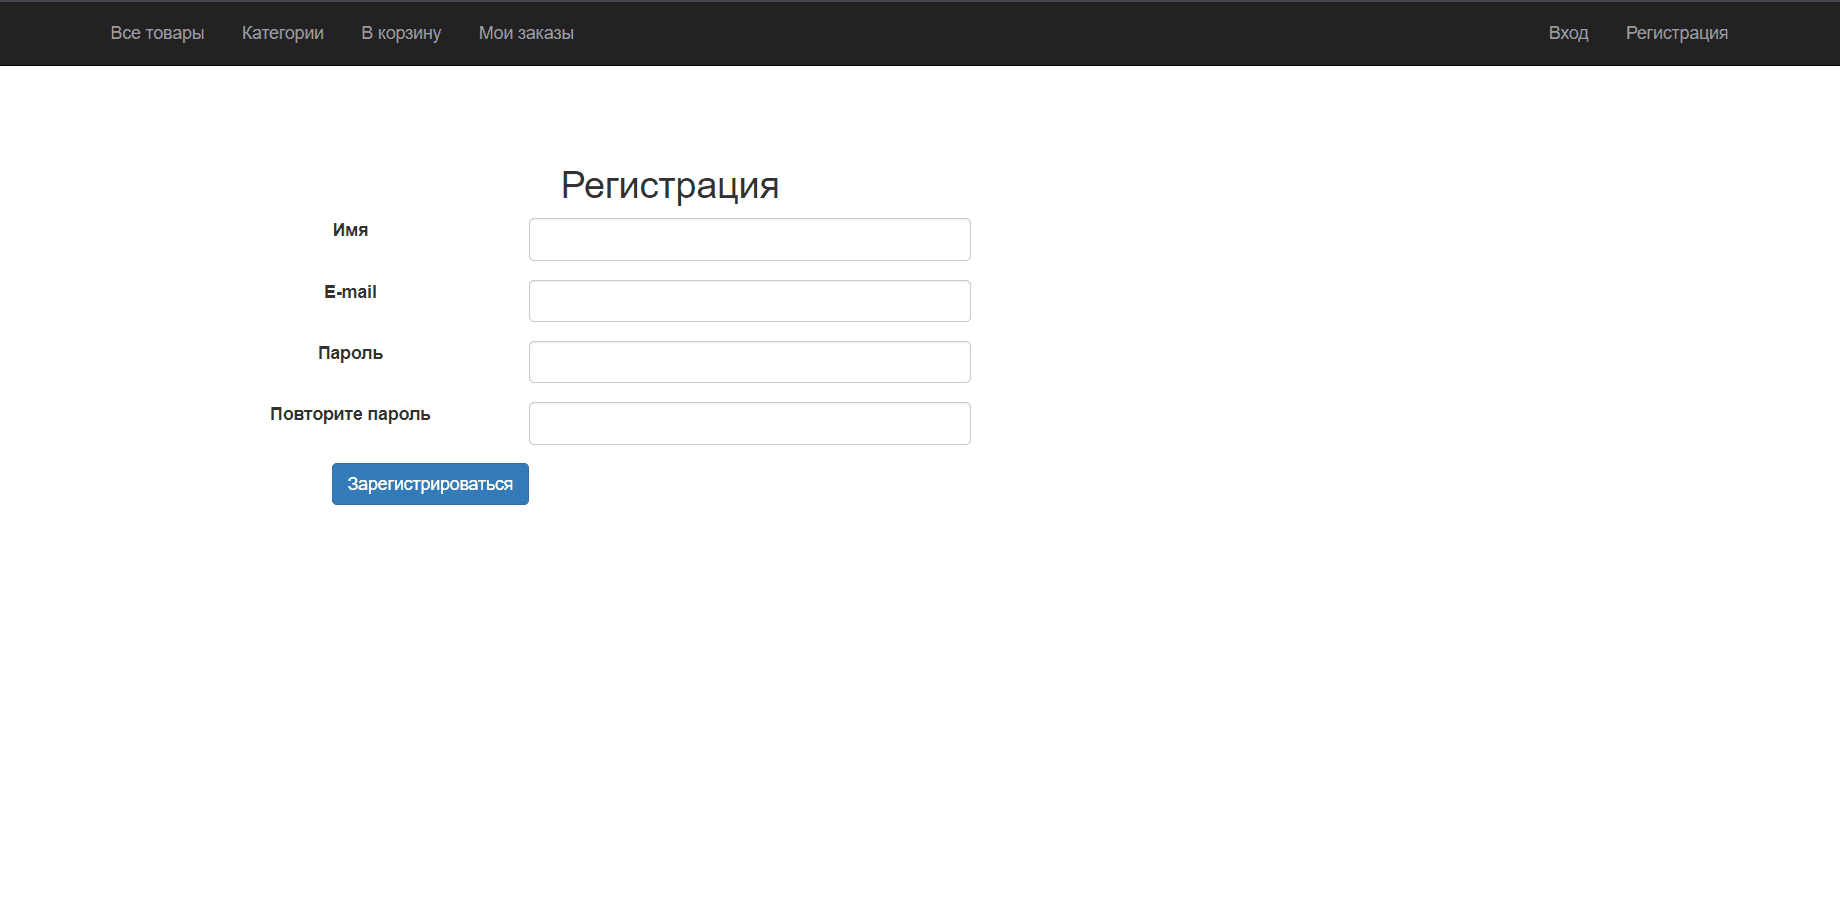
\includegraphics[width=1\linewidth]{register}
	\caption{Страница регистрации}
	\label{register:image}
\end{figure}
%\vspace{-\figureaboveskip} % двойной отступ не нужен (можно использовать, если раздел заканчивается картинкой)

На рисунке \ref{orderSuccess:image} показан результат оформления заказа.

\begin{figure}[H]
	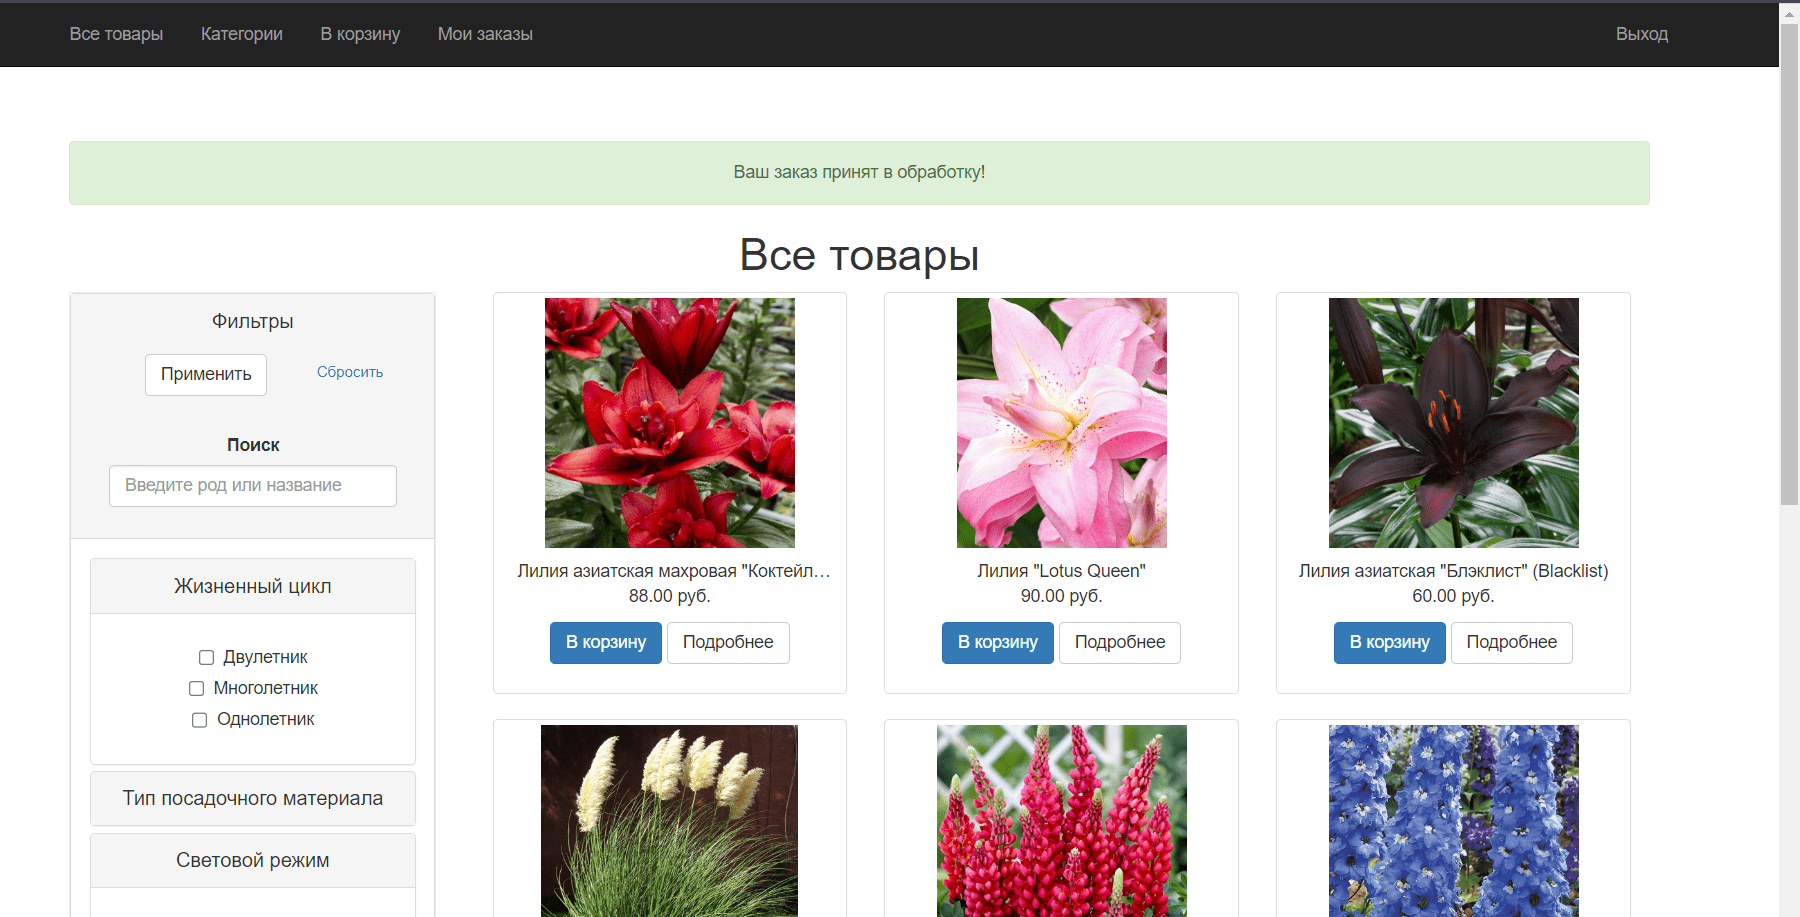
\includegraphics[width=1\linewidth]{orderSuccess}
	\caption{Результат оформления заказа}
	\label{orderSuccess:image}
\end{figure}
%\vspace{-\figureaboveskip} % двойной отступ не нужен (можно использовать, если раздел заканчивается картинкой)

На рисунке \ref{orders:image} показана страница заказов пользователя.

\begin{figure}[H]
	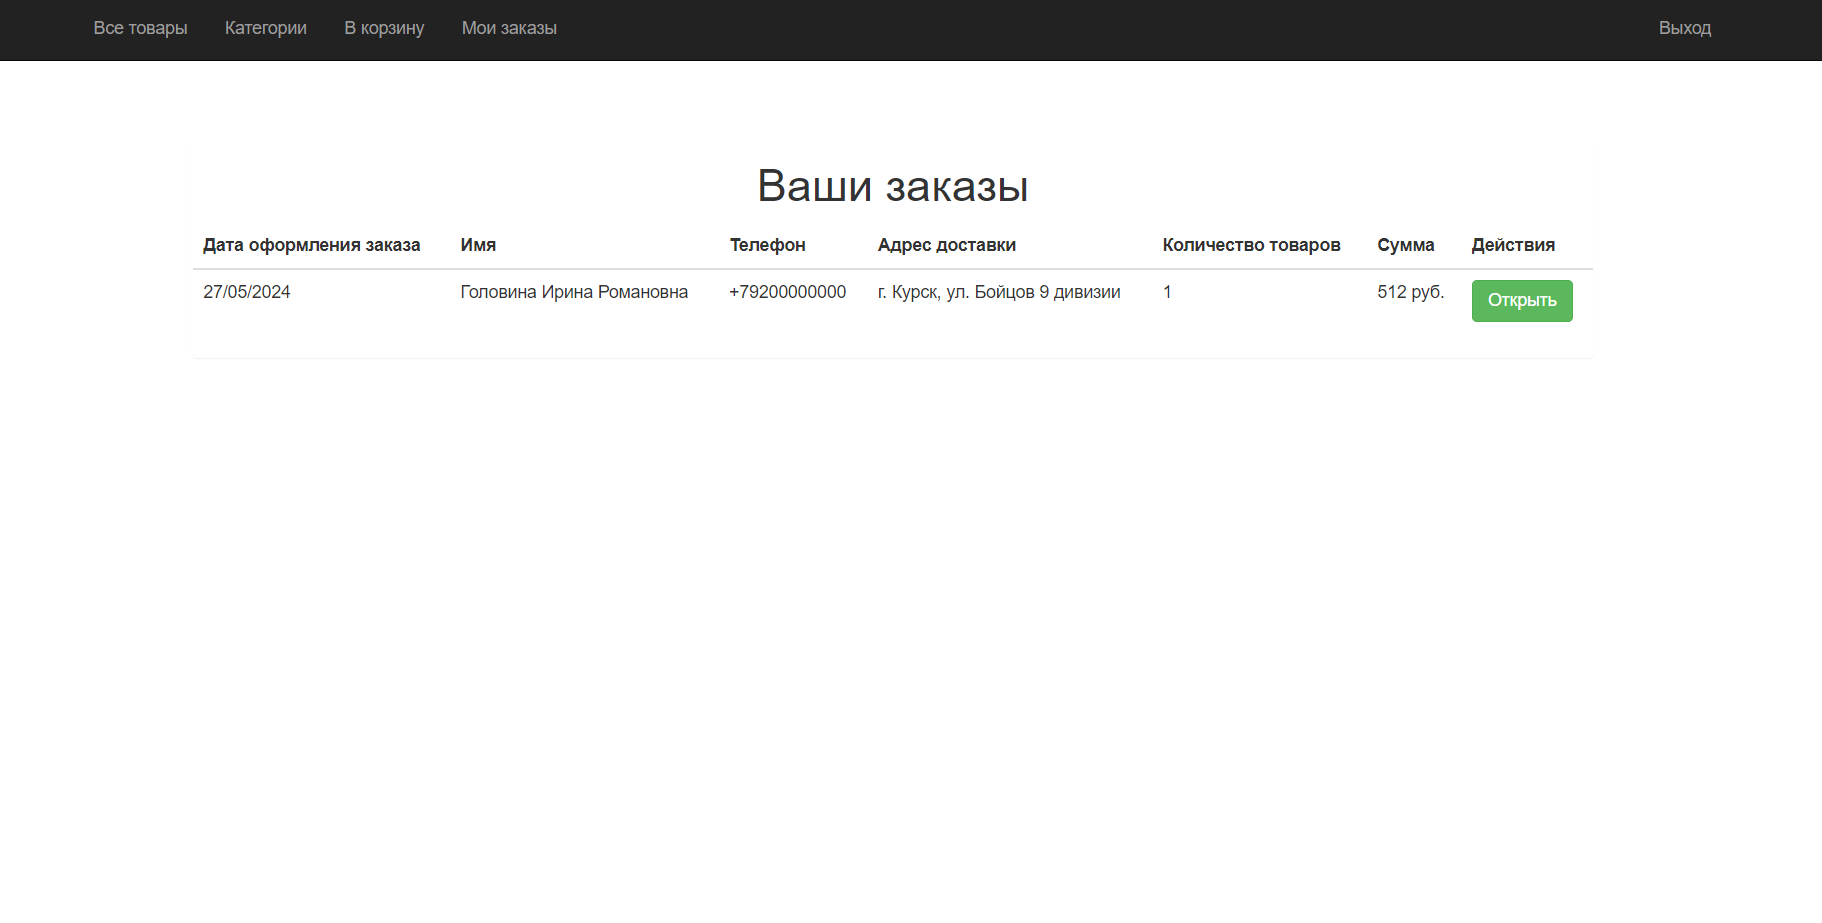
\includegraphics[width=1\linewidth]{orders}
	\caption{Страница заказов пользователя}
	\label{orders:image}
\end{figure}
%\vspace{-\figureaboveskip} % двойной отступ не нужен (можно использовать, если раздел заканчивается картинкой)

На рисунке \ref{order:image} показана страница с деталями заказа пользователя.

\begin{figure}[H]
	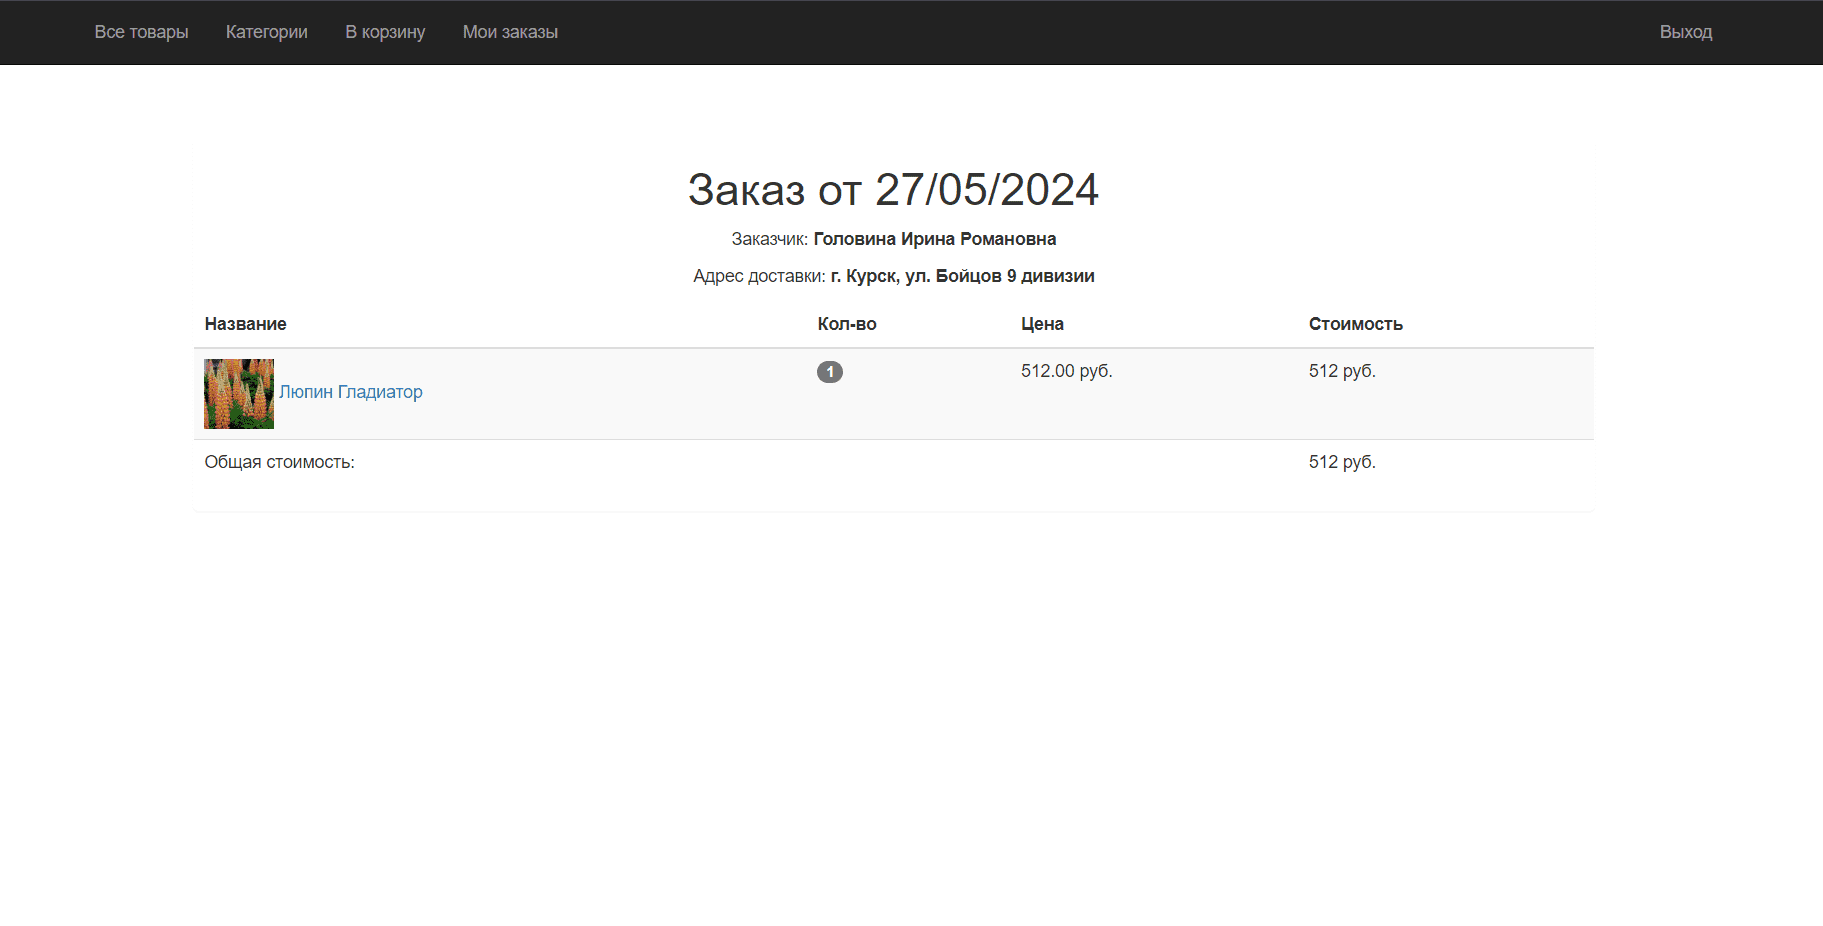
\includegraphics[width=1\linewidth]{order}
	\caption{Страница заказа пользователя}
	\label{order:image}
\end{figure}
%\vspace{-\figureaboveskip} % двойной отступ не нужен (можно использовать, если раздел заканчивается картинкой)




На рисунке \ref{ordersAdmin:image} показана страница заказов в панели администратора.

\begin{figure}[H]
	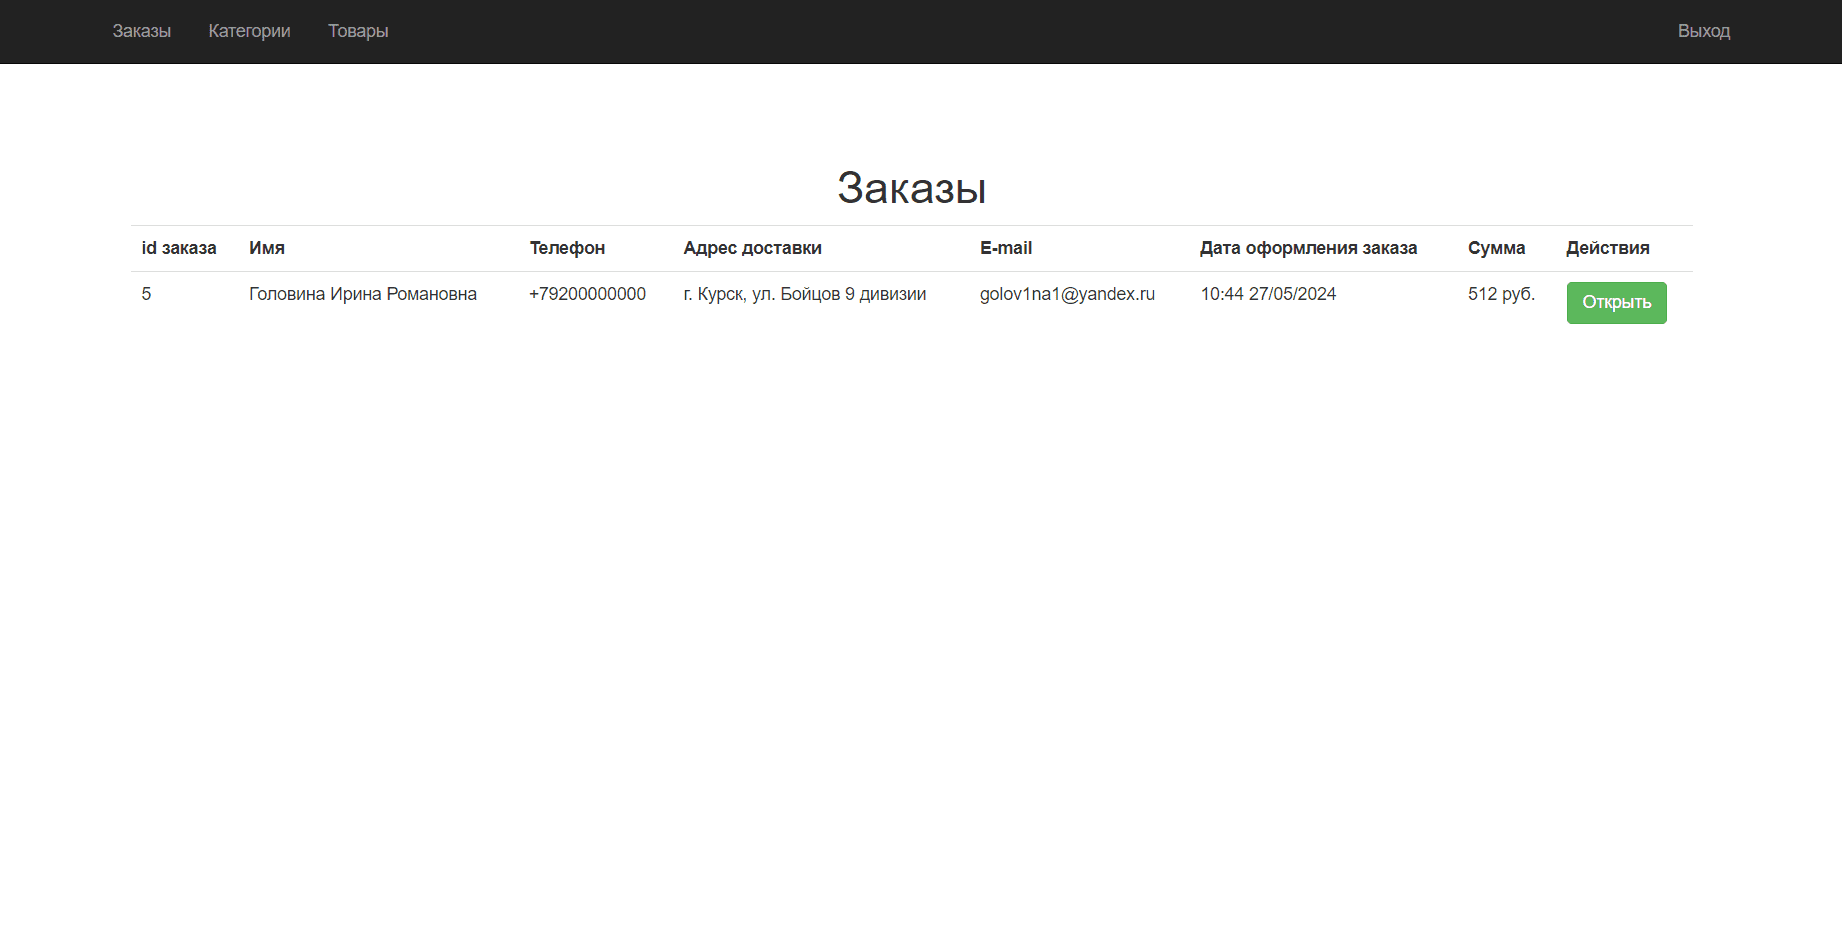
\includegraphics[width=1\linewidth]{ordersAdmin}
	\caption{Страница заказов в панели администратора}
	\label{ordersAdmin:image}
\end{figure}
%\vspace{-\figureaboveskip} % двойной отступ не нужен (можно использовать, если раздел заканчивается картинкой)

На рисунке \ref{orderAdmin:image} показана страница с деталями заказа в панели администратора.

\begin{figure}[H]
	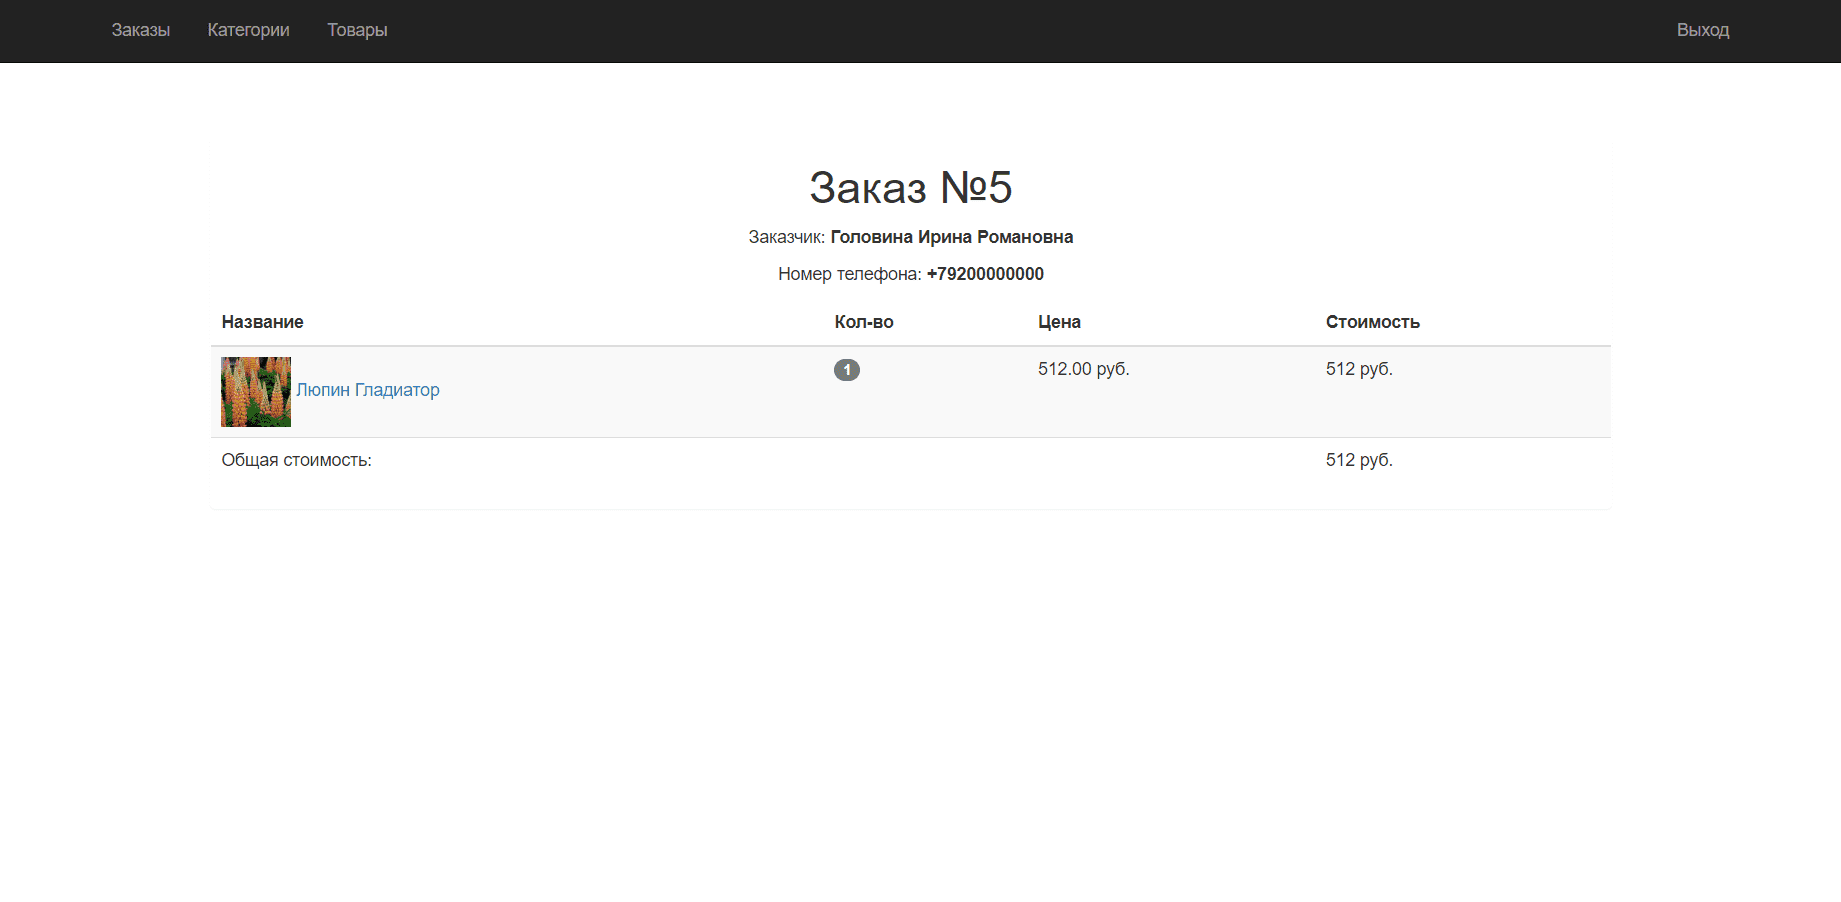
\includegraphics[width=1\linewidth]{orderAdmin}
	\caption{Страница заказа в панели администратора}
	\label{orderAdmin:image}
\end{figure}
%\vspace{-\figureaboveskip} % двойной отступ не нужен (можно использовать, если раздел заканчивается картинкой)

На рисунке \ref{categoriesAdmin:image} показана страница категорий в панели администратора.

\begin{figure}[H]
	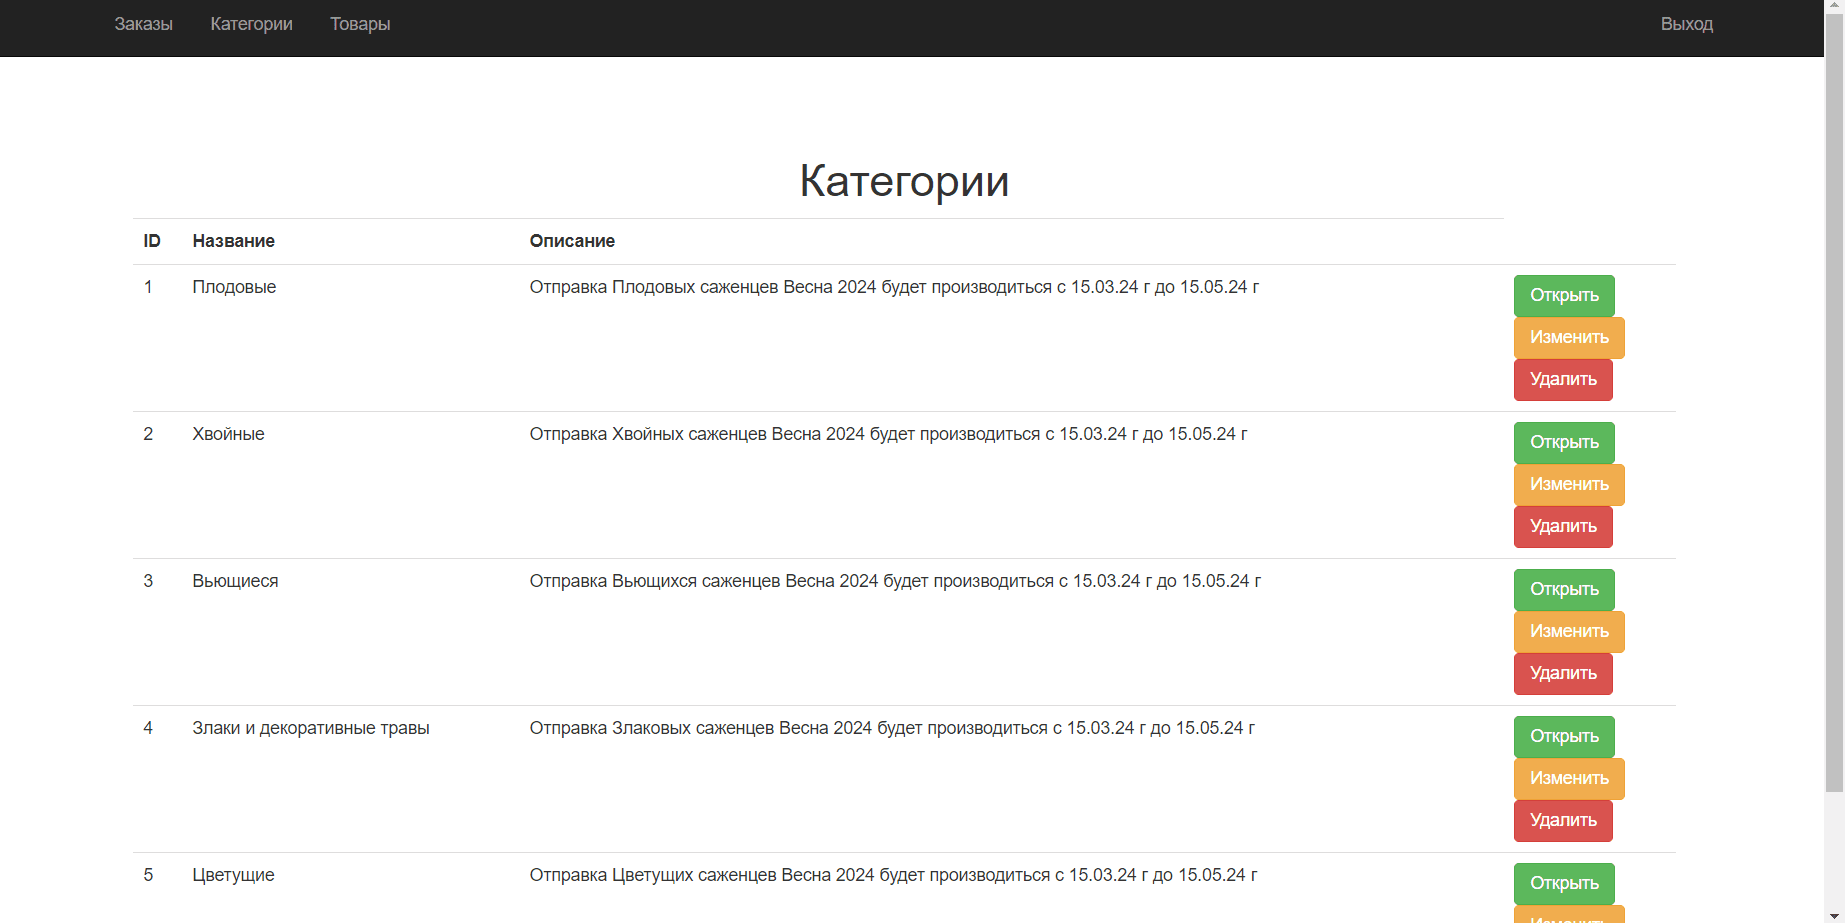
\includegraphics[width=1\linewidth]{categoriesAdmin}
	\caption{Страница категорий в панели администратора}
	\label{categoriesAdmin:image}
\end{figure}
%\vspace{-\figureaboveskip} % двойной отступ не нужен (можно использовать, если раздел заканчивается картинкой)

На рисунке \ref{categoryAdmin:image} показана страница категории <<Плодовые>> в панели администратора.

\begin{figure}[H]
	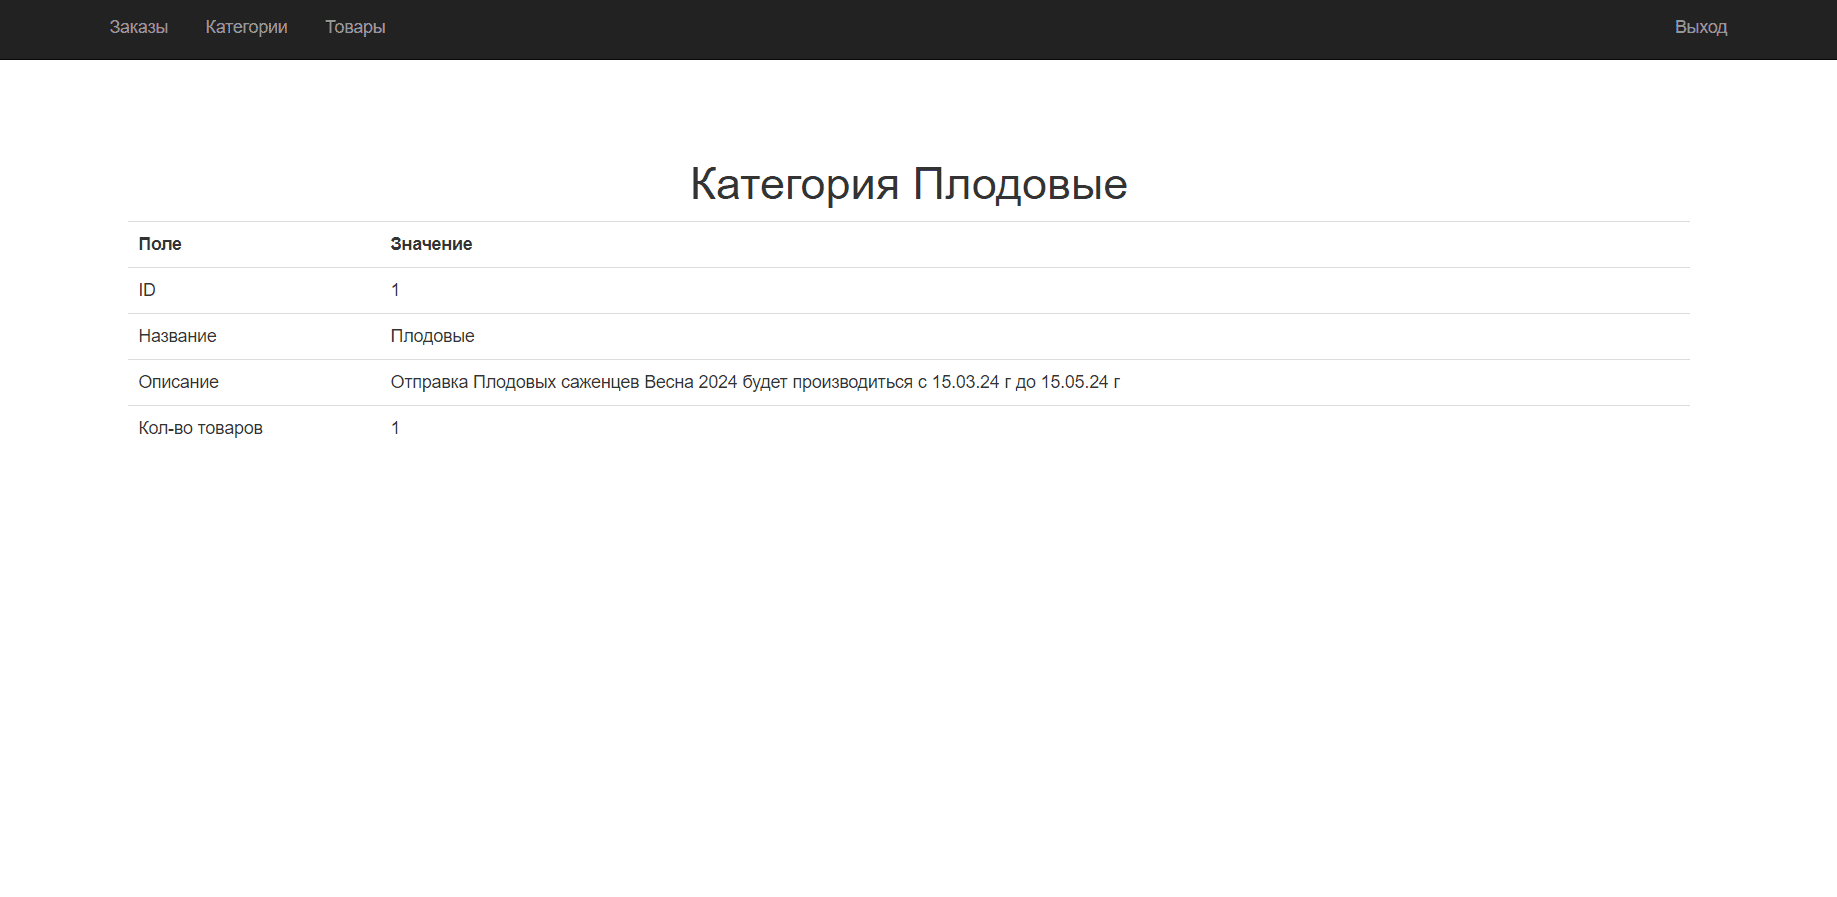
\includegraphics[width=1\linewidth]{categoryAdmin}
	\caption{Страница категории в панели администратора}
	\label{categoryAdmin:image}
\end{figure}
%\vspace{-\figureaboveskip} % двойной отступ не нужен (можно использовать, если раздел заканчивается картинкой)

На рисунке \ref{categoryEdit:image} показана страница редактирования категории <<Плодовые>> в панели администратора.

\begin{figure}[H]
	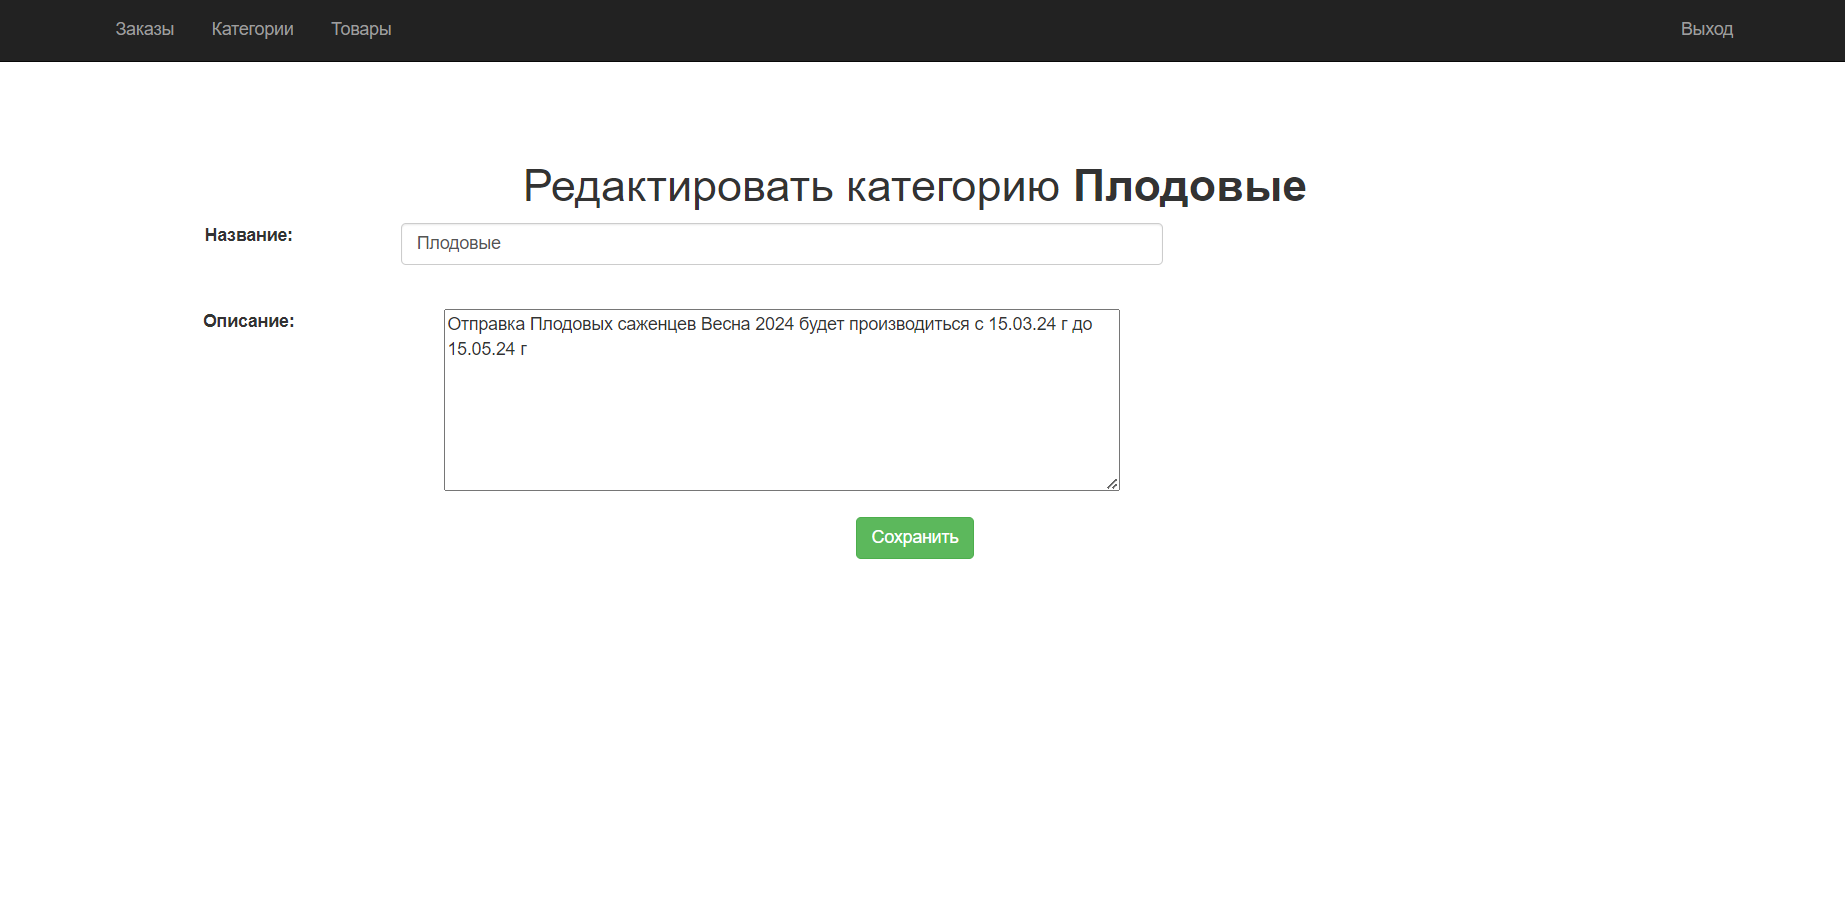
\includegraphics[width=1\linewidth]{categoryEdit}
	\caption{Страница редактирования категории в панели администратора}
	\label{categoryEdit:image}
\end{figure}
%\vspace{-\figureaboveskip} % двойной отступ не нужен (можно использовать, если раздел заканчивается картинкой)

На рисунке \ref{categoryCreate:image} показана страница создания категории в панели администратора.

\begin{figure}[H]
	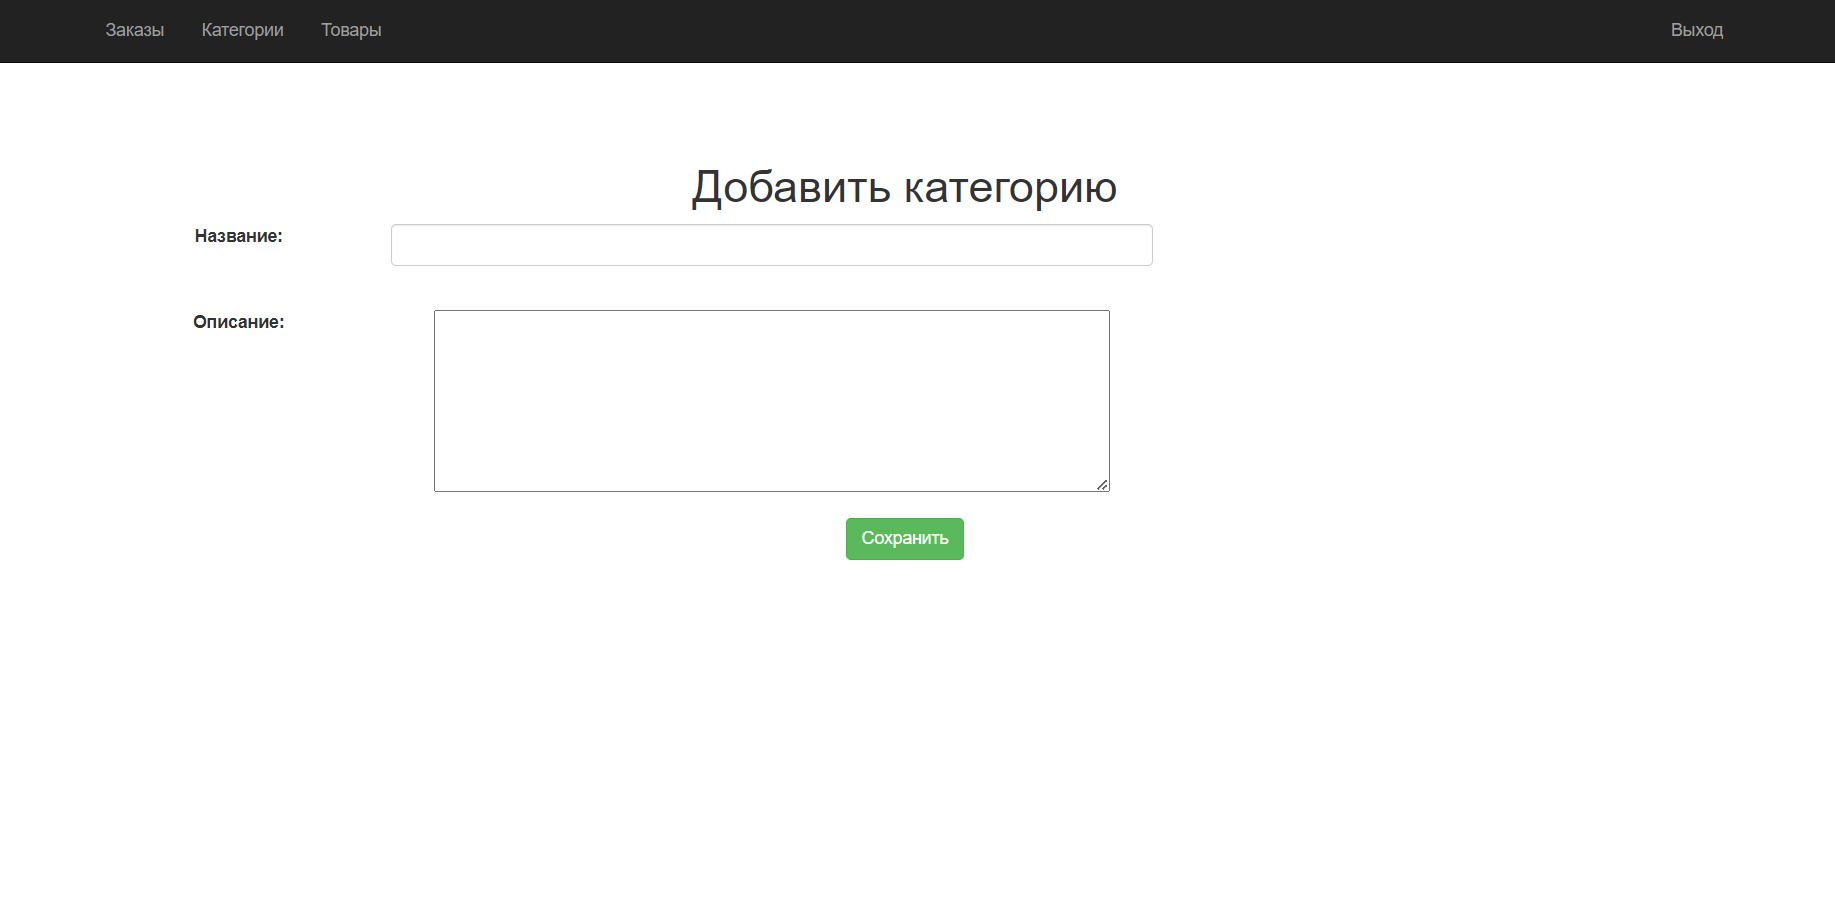
\includegraphics[width=1\linewidth]{categoryCreate}
	\caption{Страница создания категории в панели администратора}
	\label{categoryCreate:image}
\end{figure}
%\vspace{-\figureaboveskip} % двойной отступ не нужен (можно использовать, если раздел заканчивается картинкой)


На рисунке \ref{productsAdmin:image} показана страница товаров в панели администратора.

\begin{figure}[H]
	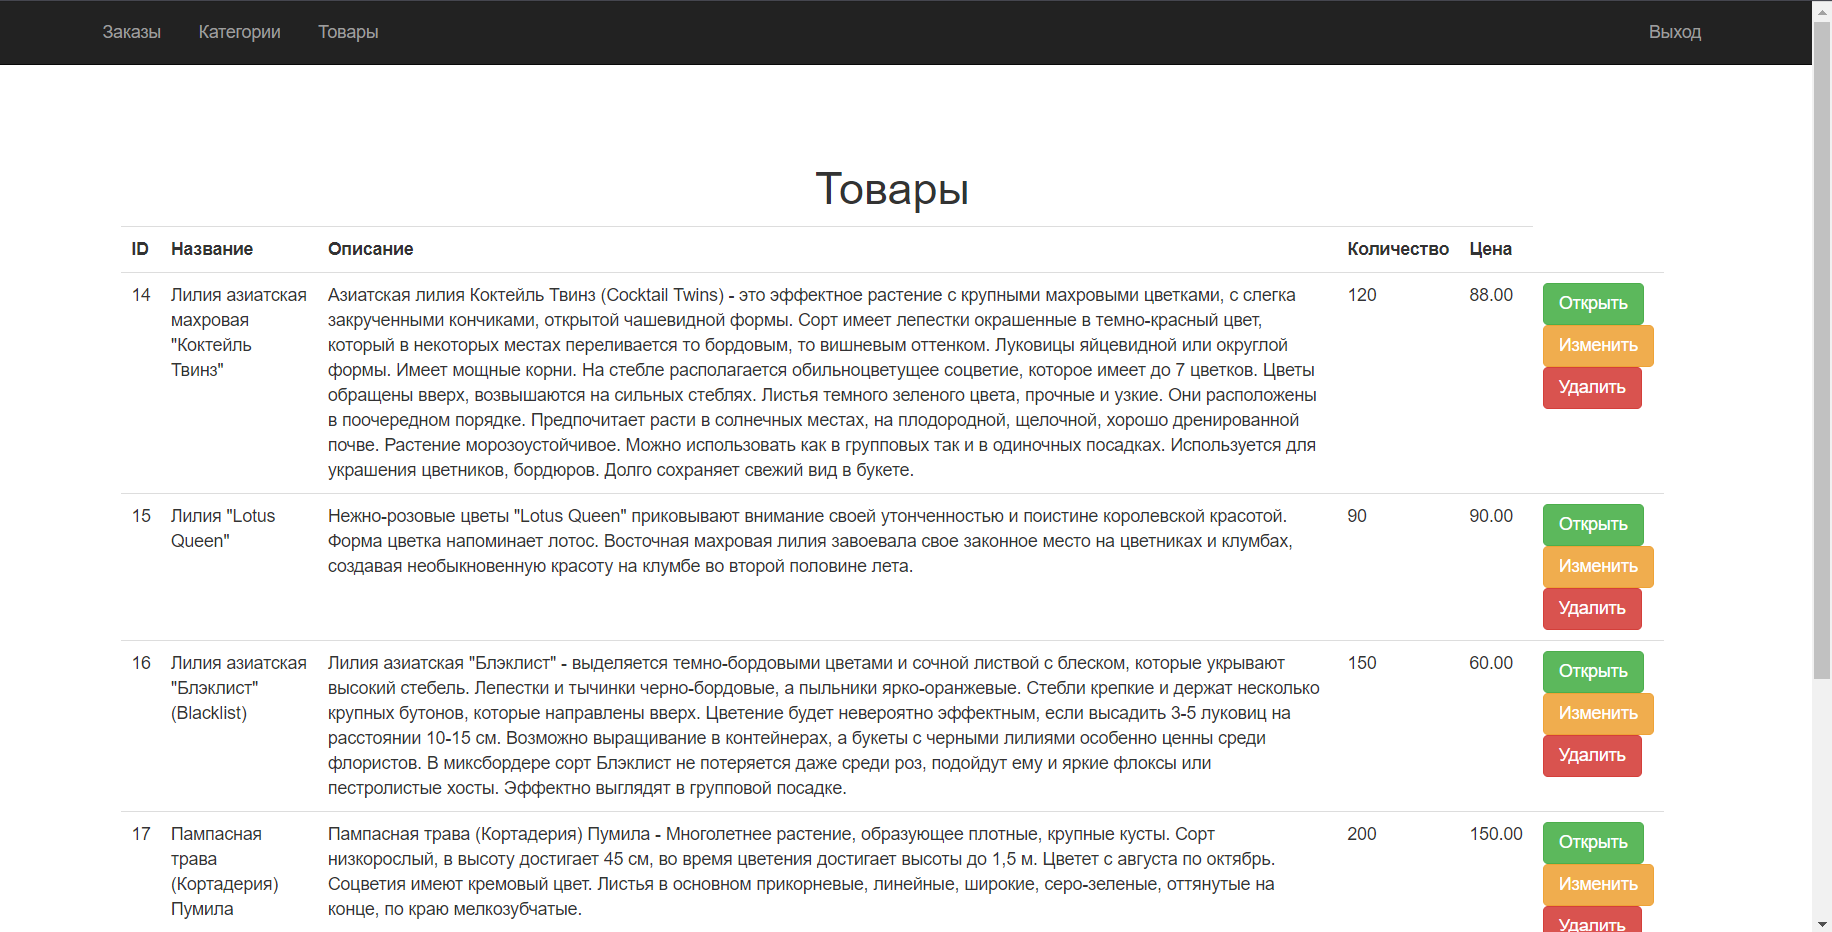
\includegraphics[width=1\linewidth]{productsAdmin}
	\caption{Страница товаров в панели администратора}
	\label{productsAdmin:image}
\end{figure}
%\vspace{-\figureaboveskip} % двойной отступ не нужен (можно использовать, если раздел заканчивается картинкой)

На рисунке \ref{productAdmin:image} показана страница одного из товаров в панели администратора.

\begin{figure}[H]
	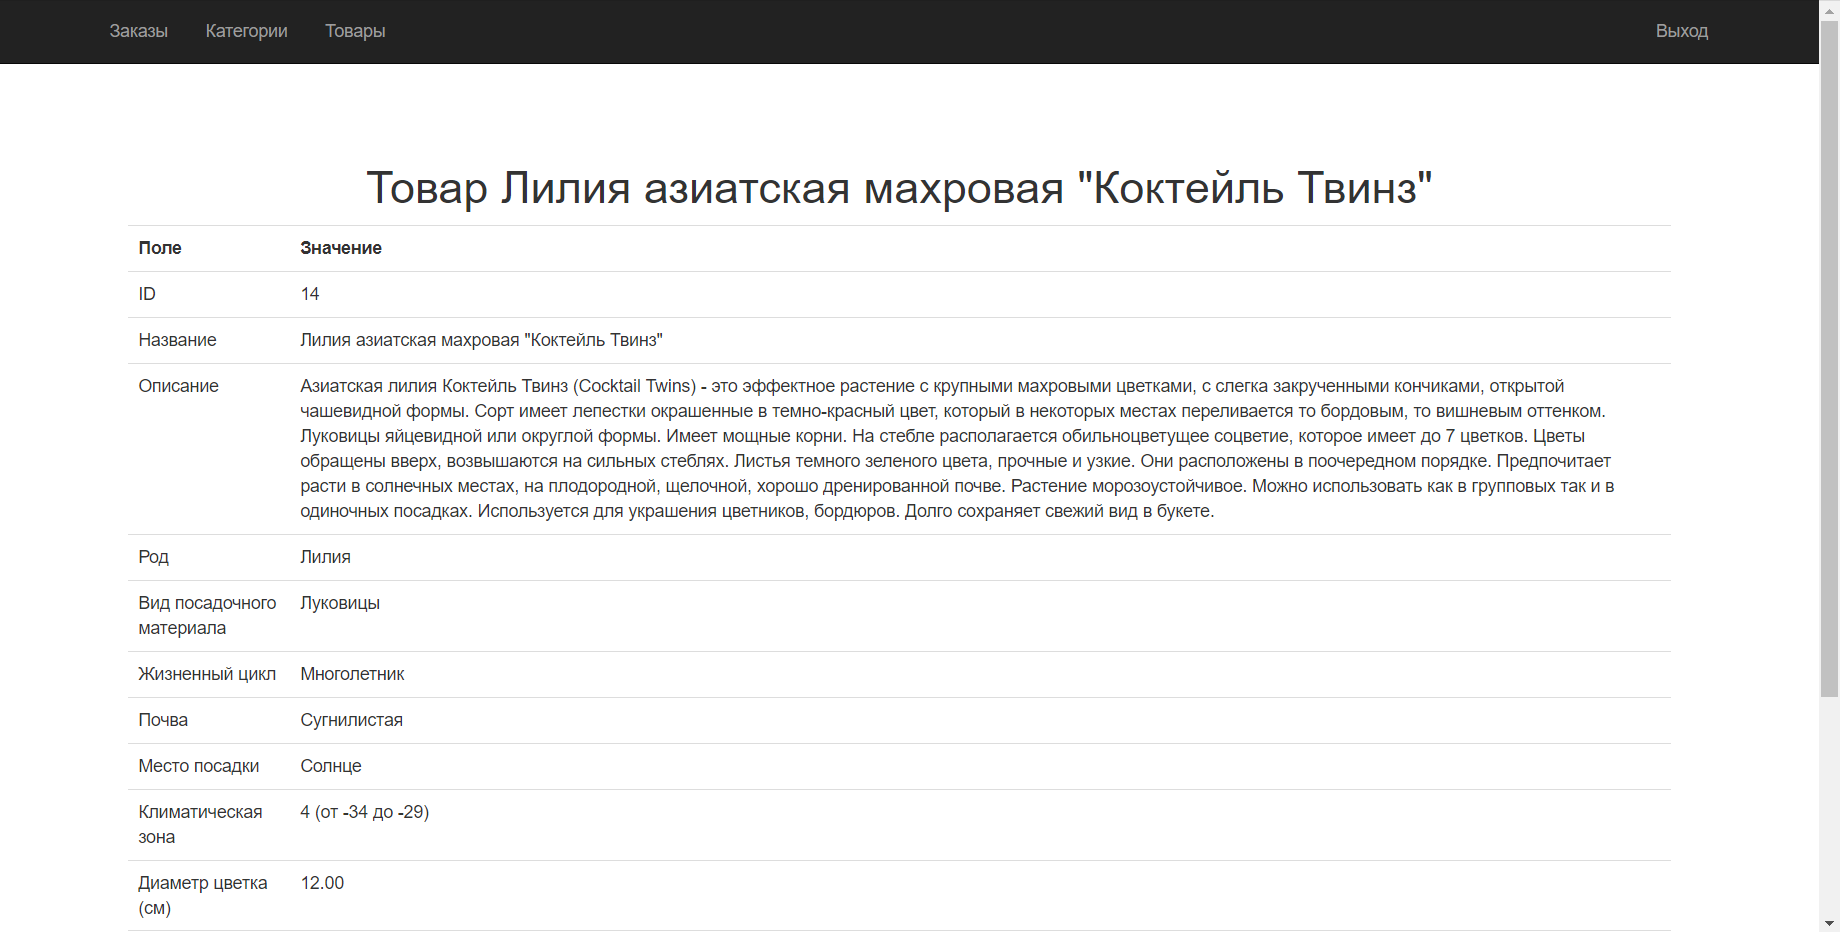
\includegraphics[width=1\linewidth]{productAdmin}
	\caption{Страница товара в панели администратора}
	\label{productAdmin:image}
\end{figure}
%\vspace{-\figureaboveskip} % двойной отступ не нужен (можно использовать, если раздел заканчивается картинкой)

На рисунке \ref{productEdit:image} показана страница редактирования товара в панели администратора.

\begin{figure}[H]
	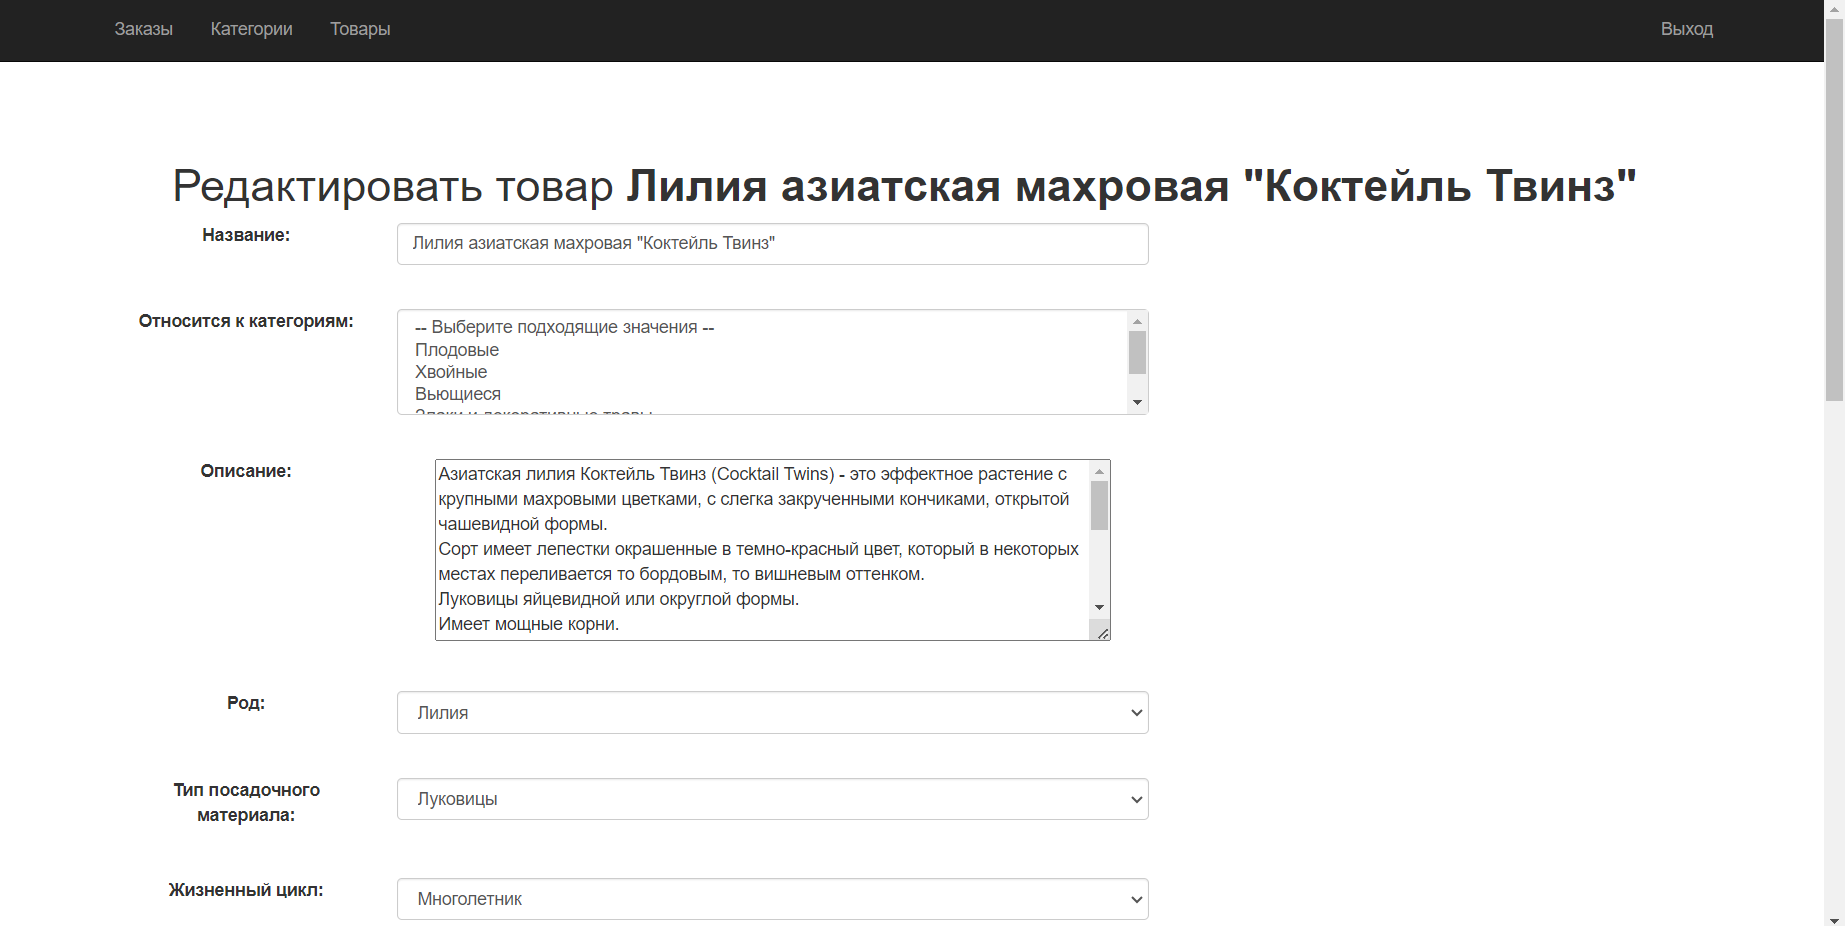
\includegraphics[width=1\linewidth]{productEdit}
	\caption{Страница редактирования товара в панели администратора}
	\label{productEdit:image}
\end{figure}
%\vspace{-\figureaboveskip} % двойной отступ не нужен (можно использовать, если раздел заканчивается картинкой)

На рисунке \ref{productCreate:image} показана страница создания товара в панели администратора.

\begin{figure}[H]
	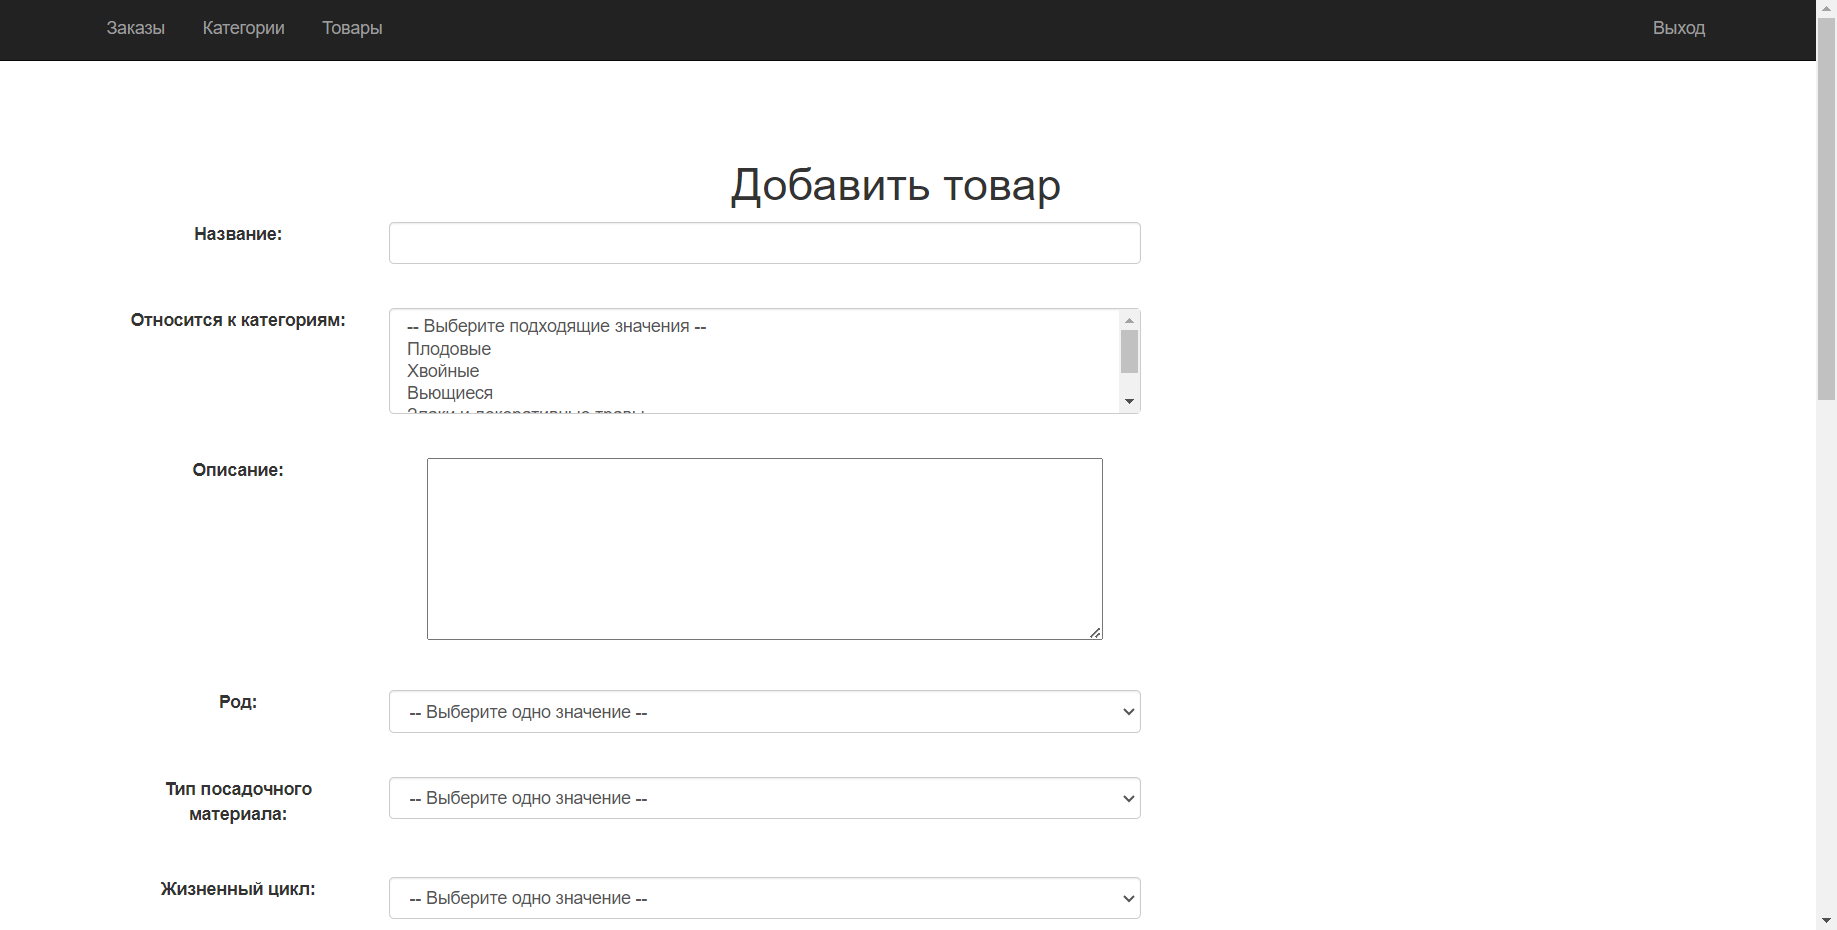
\includegraphics[width=1\linewidth]{productCreate}
	\caption{Страница создания товара в панели администратора}
	\label{productCreate:image}
\end{figure}
%\vspace{-\figureaboveskip} % двойной отступ не нужен (можно использовать, если раздел заканчивается картинкой)


